
    \chapter{Vectors}
    \section*{Introduction}
        Often times a single number is not adequate for describing a quantity.  Take for example, velocity.  In order to describe the velocity of a particle, we need to know the direction in space the particle travels along with its speed.  This takes three numbers to describe (since we move in a 3-dimensional space). Compare this to temperature.  At any given point in space, we can describe the temperature with a single number. 
        
        \section{Vectors and Scalars}
        
        We then say the following:
        
        \begin{df}{Scalar}{scalar}
        A \textbf{scalar} \index{scalar} quantity is described by a single number.  
        \end{df}
        
        \begin{df}{Vector}{vector}
        A \textbf{vector} \index{vector} quantity is described by $n$ numbers. 
        \end{df}
        
        We usually represent a vector $\mathbf{v}$ as an arrow starting with a tail at the origin ($\mathbf{0}$), and head at the desired point.  
        
        \begin{center}
        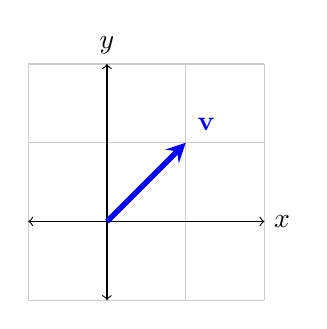
\begin{tikzpicture}
        \draw[thin,gray!40] (-1,-1) grid (2,2);
        \draw[<->] (-1,0)--(2,0) node[right]{$x$};
        \draw[<->] (0,-1)--(0,2) node[above]{$y$};
        \draw[line width=2pt,blue,-stealth](0,0)--(1,1) node[anchor=south west]{$\mathbf{v}$};
        \end{tikzpicture}
        \end{center}
        
        Here in this case we would write $\mathbf{v}=(1,1)$ as the head of the arrow lies where $x=1$ and $y=1$. We should also write, $\mathbf{0}=(0,0)$. More on this notation later.
        
        \begin{ex}{Position of an Object}{position}
        If you are measuring the position of an object $P$ relative to yourself $O$ ($O$ for \emph{origin}), we can describe this with a vector.  We write $\mathbf{p}=\overrightarrow{OP}$ to signify the arrow with the tail at your eyes and head on the object. 
        
        
\begin{center}
\tdplotsetmaincoords{60}{120} 
\begin{tikzpicture} [scale=3, tdplot_main_coords, axis/.style={->,black,thick}, 
vector/.style={-stealth,blue,very thick}, 
vector guide/.style={dashed,red,thick}]

%standard tikz coordinate definition using x, y, z coords
\coordinate (O) at (0,0,0);

%tikz-3dplot coordinate definition using x, y, z coords

\pgfmathsetmacro{\ax}{0.6}
\pgfmathsetmacro{\ay}{1}
\pgfmathsetmacro{\az}{0.8}

\coordinate (P) at (\ax,\ay,\az);

%draw axes
\draw[axis] (0,0,0) -- (1,0,0) node[anchor=north east]{$x$};
\draw[axis] (0,0,0) -- (0,1,0) node[anchor=north west]{$y$};
\draw[axis] (0,0,0) -- (0,0,1) node[anchor=south]{$z$};

%draw a vector from O to P
\draw[vector] (O) -- (P) node[anchor=south east] at (.3,.5,.4){$\mathbf{p}$};

%draw guide lines to components
\draw[vector guide]         (O) -- (\ax,\ay,0);
\draw[vector guide] (\ax,\ay,0) -- (P);
\draw[vector guide]         (P) -- (0,0,\az);
\draw[vector guide] (\ax,\ay,0) -- (0,\ay,0);
\draw[vector guide] (\ax,\ay,0) -- (0,\ay,0);
\draw[vector guide] (\ax,\ay,0) -- (\ax,0,0);
\node[tdplot_main_coords,anchor=east]
at (\ax,0,0){};
\node[tdplot_main_coords,anchor=west]
at (0,\ay,0){};
\node[tdplot_main_coords,anchor=south]
at (0,0,\az){};
\node[tdplot_main_coords, anchor=east] at (0,0,0){$O$};
\node[tdplot_main_coords, anchor=west] at (\ax,\ay,\az){$P$};
\end{tikzpicture}
\end{center}

        If $P$ moves over time, then our vector $\mathbf{p}$ changes over time as well. We'll often denote this $\mathbf{p}(t)$.  It's possible the position of an object changes due to interactions with the environment or other objects.  All to come later.

        \end{ex}
        
        Great, we have some objects, but what can we do with them?  As it turns out, we can do quite a bit.  For the most part, anything we could do with numbers, we can do with vectors.  However, we have to be comfortable looking at things in new ways.
        
        \section{Vector Algebra}
        
        Our first vector operation is \textbf{vector addition}.  Given two vectors $\mathbf{a}$ and $\mathbf{b}$, we can create a new vector
        \[
        \mathbf{c}=\mathbf{a}+\mathbf{b}.
        \]
        Addition is a commutative operation and so we also have that
        \[
        \mathbf{c}=\mathbf{b}+\mathbf{a}.
        \]
        Pictorially, what do we do when we add vectors? We take $\mathbf{a}$ and attach the tail of $\mathbf{b}$ to the head $\mathbf{a}$. 
        
        \begin{center}
        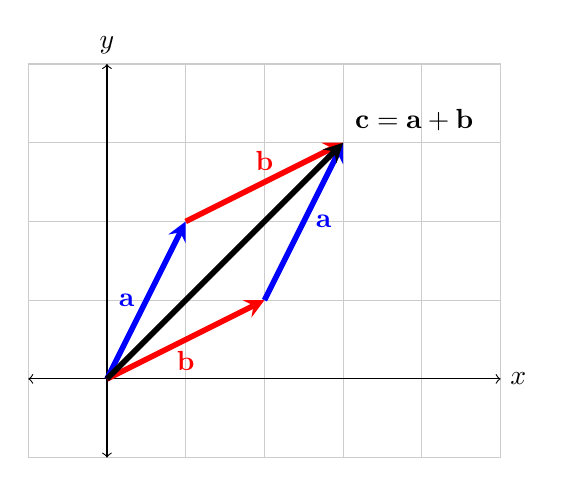
\begin{tikzpicture}
        \draw[thin,gray!40] (-1,-1) grid (5,4);
        \draw[<->] (-1,0)--(5,0) node[right]{$x$};
        \draw[<->] (0,-1)--(0,4) node[above]{$y$};
        \draw[line width=2pt,blue,-stealth](0,0)--(1,2) node[anchor=east] at (.5,1){$\mathbf{a}$};
        \draw[line width=2pt, red, -stealth](0,0)--(2,1) node[anchor=north] at (1,.5){$\mathbf{b}$};
        \draw[line width=2pt, red, -stealth](1,2)--(3,3) node[anchor=south] at (2,2.5){$\mathbf{b}$};
        \draw[line width=2pt, blue, -stealth](2,1)--(3,3) node[anchor=west] at (2.5,2){$\mathbf{a}$};
        \draw[line width=2pt, black, -stealth](0,0)--(3,3) node[anchor=south west]{$\mathbf{c}=\mathbf{a}+\mathbf{b}$};
        \end{tikzpicture}
        \end{center}
        
        From this diagram, you can see why the operation is commutative.  Both paths, $\mathbf{a}+\mathbf{b}$ and $\mathbf{b}+\mathbf{a}$, lead to the same $\mathbf{c}$.
        
        
        As always, repeated addition gives us a form of multiplication. What will this mean here? 
        
        \begin{exercise}
        Draw a 2-dimensional coordinate system ($x$ and $y$ axes), and draw some vector $\mathbf{a}$.  Using vector addition, what does $\mathbf{a}+\mathbf{a}=2\mathbf{a}$ look like? Given this, what do you think $\frac{1}{2}\mathbf{a}$ will look like? 
        \end{exercise}
        
        When dealing with a vector, we are allowed to scale the length.  We call this \textbf{scalar multiplication}. Since the vector $2\mathbf{a}$ has twice the length of $\mathbf{a}$, we would expect $\frac{1}{2} \mathbf{a}$ to have half the length of $\mathbf{a}$.  All of these vectors point in the same direction though.  We have merely scaled their lengths.
        
        \begin{question}
        What happens if we take $-\mathbf{a}$ (i.e., $-1\cdot \mathbf{a}$)? \emph{Hint: Consider what happens for numbers on a number line when multiplied by $-1$.} 
        \end{question}
        
        \begin{answer}
        It flips the direction of the vector.
        \end{answer}
        
        We can take a look at all of this. 
        
        \begin{center}
        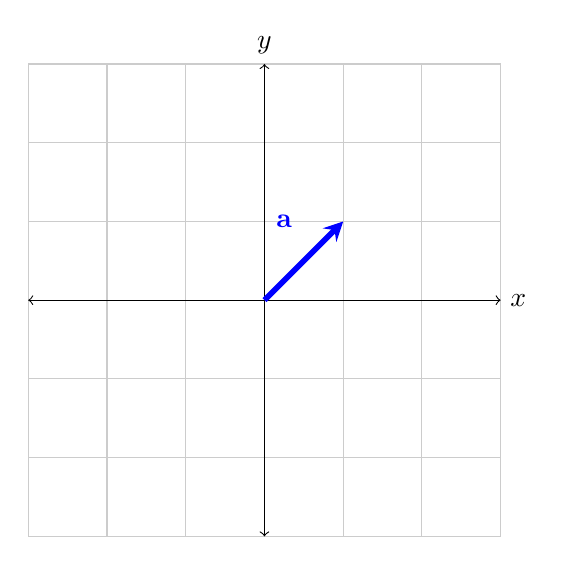
\begin{tikzpicture}
        \draw[thin,gray!40] (-3,-3) grid (3,3);
        \draw[<->] (-3,0)--(3,0) node[right]{$x$};
        \draw[<->] (0,-3)--(0,3) node[above]{$y$};
        \draw[line width=2pt,blue,-stealth](0,0)--(1,1) node[anchor=east] at (.5,1){$\mathbf{a}$};
        \end{tikzpicture}
        \qquad
        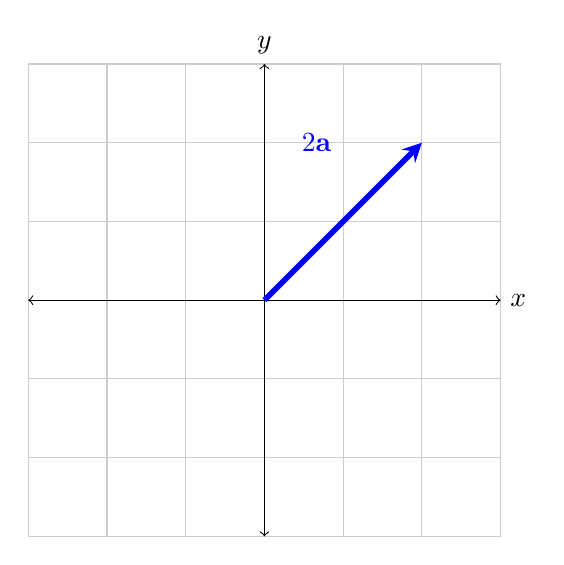
\begin{tikzpicture}
        \draw[thin,gray!40] (-3,-3) grid (3,3);
        \draw[<->] (-3,0)--(3,0) node[right]{$x$};
        \draw[<->] (0,-3)--(0,3) node[above]{$y$};
        \draw[line width=2pt,blue,-stealth](0,0)--(2,2) node[anchor=east] at (1,2){$2\mathbf{a}$};
        \end{tikzpicture}
        
        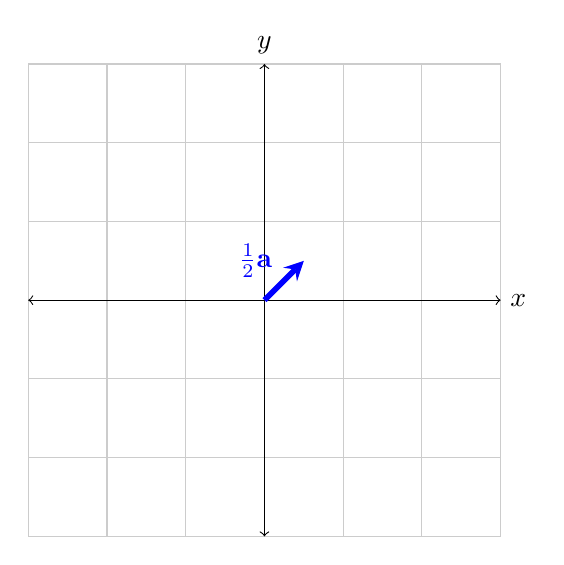
\begin{tikzpicture}
        \draw[thin,gray!40] (-3,-3) grid (3,3);
        \draw[<->] (-3,0)--(3,0) node[right]{$x$};
        \draw[<->] (0,-3)--(0,3) node[above]{$y$};
        \draw[line width=2pt,blue,-stealth](0,0)--(.5,.5) node[anchor=east] at (.25,.5){$\frac{1}{2}\mathbf{a}$};
        \end{tikzpicture}
        \qquad
        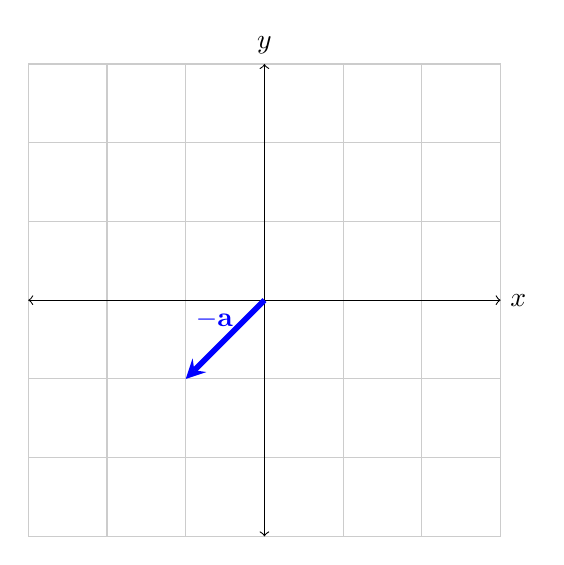
\begin{tikzpicture}
        \draw[thin,gray!40] (-3,-3) grid (3,3);
        \draw[<->] (-3,0)--(3,0) node[right]{$x$};
        \draw[<->] (0,-3)--(0,3) node[above]{$y$};
        \draw[line width=2pt,blue,-stealth](0,0)--(-1,-1) node[anchor=east] at (-.25,-.25){$-\mathbf{a}$};
        \end{tikzpicture}
        \end{center}
        
        \begin{question}
        How can we go about defining $\mathbf{a}-\mathbf{b}$?  
        \end{question}
        
        \begin{answer}
        We can write $\mathbf{a}+(-\mathbf{b})$ and use the rules for vector addition and scalar multiplication together.
        \end{answer}
        
        \begin{exercise}
        Draw two different vectors $\mathbf{a}$ and $\mathbf{b}$ and draw the following:
        \begin{itemize}
            \item $\mathbf{a}+\mathbf{b}$,
            \item $\mathbf{a}-\mathbf{b}$,
            \item $\mathbf{b}-\mathbf{a}$.
        \end{itemize}
        \end{exercise}
        
        Now see the picture below.
        
        \begin{center}
        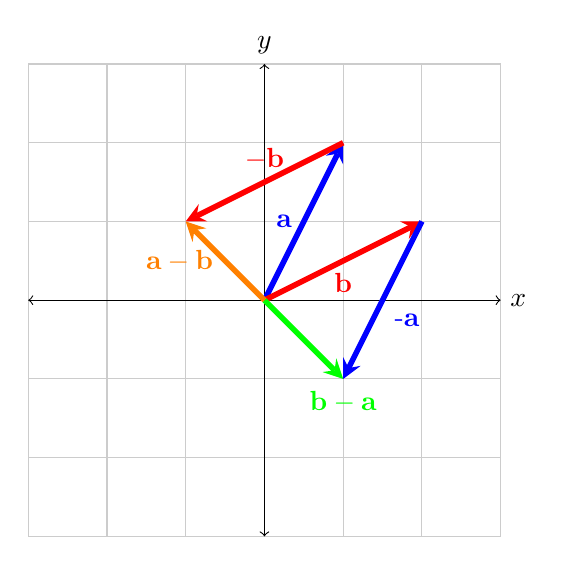
\begin{tikzpicture}
        \draw[thin,gray!40] (-3,-3) grid (3,3);
        \draw[<->] (-3,0)--(3,0) node[right]{$x$};
        \draw[<->] (0,-3)--(0,3) node[above]{$y$};
        \draw[line width=2pt,blue,-stealth](0,0)--(1,2) node[anchor=east] at (.5,1){$\mathbf{a}$};
        \draw[line width=2pt, red, -stealth](0,0)--(2,1) node[anchor=north] at (1,.5){$\mathbf{b}$};
        \draw[line width=2pt, red, -stealth](1,2)--(-1,1) node[anchor=south] at (0,1.5){$-\mathbf{b}$};
        \draw[line width=2pt, blue, -stealth](2,1)--(1,-1) node[anchor=west] at (1.5,-.25){-$\mathbf{a}$};
        \draw[line width=2pt, green, -stealth](0,0)--(1,-1) node[anchor=north]{$\mathbf{b}-\mathbf{a}$};
        \draw[line width=2pt, orange, -stealth](0,0)--(-1,1) node[anchor=east] at (-.5,.5){$\mathbf{a}-\mathbf{b}$};
        \end{tikzpicture}
        \end{center}
        
        
        \section{Vector Components}
        To work with vectors more effectively, it's necessary to break them down into \textbf{components}. Let us consider the following.
        
        \begin{ex}{Components of a Vector}{vector_components}
        Let us fix an arbitrary vector $\mathbf{a}$ in $\R^2$ (i.e., the $xy$-plane).  
        \begin{center}
        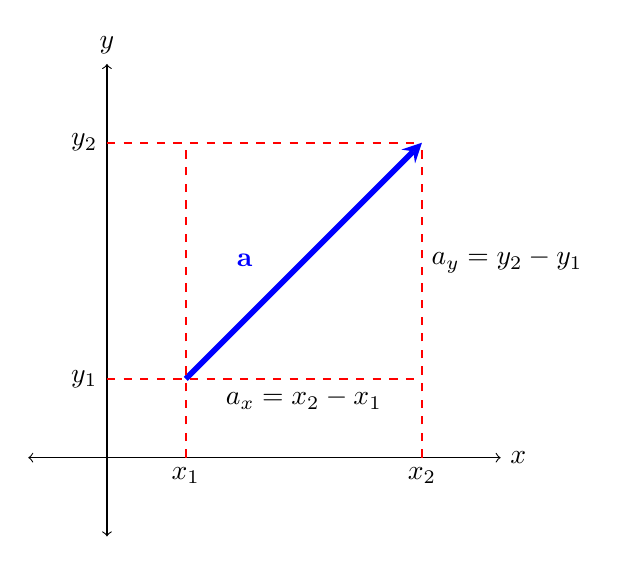
\begin{tikzpicture}[vector guide/.style={dashed,red,thick}]
        \draw[<->] (-1,0)--(5,0) node[right]{$x$};
        \draw[<->] (0,-1)--(0,5) node[above]{$y$};
        \draw[line width=2pt,blue,-stealth](1,1)--(4,4) node[anchor=east] at (2,2.5){$\mathbf{a}$};
        \draw[vector guide] (1,0) -- (1,4);
        \draw[vector guide] (4,0) -- (4,4);
        \draw[vector guide] (0,1) -- (4,1);
        \draw[vector guide] (0,4) -- (4,4);
        \node[anchor=north] at (1,0){$x_1$};
        \node[anchor=north] at (4,0){$x_2$};
        \node[anchor=east] at (0,1){$y_1$};
        \node[anchor=east] at (0,4){$y_2$};
        \node[anchor=north] at (2.5,1){$a_x=x_2-x_1$};
        \node[anchor=west] at (4,2.5){$a_y=y_2-y_1$};
        \end{tikzpicture}
        \end{center}
        We can break down this vector into the portions that are in the $x$-direction and $y$-direction.  We say that the component of the vector in the $x$-direction is $a_x=x_2-x_1$ and the component of the vector in the $y$-direction is $a_y=y_2-y_1$.  It follows that the length of the vector is $|\mathbf{a}|=\sqrt{a_x^2+a_y^2}$ and the direction is the slope $a_y/a_x$. 
        
        We often write vectors in the following way 
        \[
        \mathbf{a}=(a_x,a_y).
        \]
        \end{ex} 
        
        
        \subsubsection{Unit Coordinate Vectors}
        Another way of writing a vector $\mathbf{a}$ is as follows. We create unit vectors $\hat{\mathbf{\i}}=(1,0)$ and $\hat{\mathbf{\j}}=(0,1)$. 
        \begin{center}
        \begin{tikzpicture}[vector guide/.style={dashed,red,thick}]
        \draw[<->] (-1,0)--(3,0) node[right]{$x$};
        \draw[<->] (0,-1)--(0,3) node[above]{$y$};
        \draw[line width=2pt,blue,-stealth](0,0)--(1,0) node[anchor=north] at (1,0){$\mathbf{\hat{\i}}$};
        \draw[line width=2pt, red,-stealth](0,0)--(0,1) node[anchor=east] at (0,1){$\mathbf{\hat{\j}}$};
        \end{tikzpicture}
        \end{center}
        Then another way of writing $\mathbf{a}$ is
        \[
        \mathbf{a}=a_x \mathbf{\hat{\i}}+a_y\mathbf{\hat{\j}}.
        \]

        
        When working in 3-dimensions, we typically use the unit vectors
        \begin{align*}
            \mathbf{\hat{\i}}&=(1,0,0)\\
            \mathbf{\hat{\j}}&=(0,1,0)\\
            \mathbf{\hat{k}}&=(0,0,1).
        \end{align*}
        Sometimes others write
        \begin{align*}
            \mathbf{\hat{\i}}&=\mathbf{\hat{x}}\\
            \mathbf{\hat{\j}}&=\mathbf{\hat{y}}\\
            \mathbf{\hat{k}}&=\mathbf{\hat{z}}.
        \end{align*}

    \section{Vector Algebra with Components}
        It is helpful to think of vectors as an ordered list of numbers. Why? Well, if two ordered lists are to be equal, then each part of the list must also be equal. \begin{enumerate}[(i)]
            \item \textbf{Equality:} Vectors are equal when their components are equal,
            \[
            \mathbf{a}=\mathbf{b} ~~ \textrm{if} ~~ a_x+b_x, ~~ a_y=b_y ~~ \textrm{and} ~~ a_z=b_z.
            \]
            \item \textbf{Addition:} The sum $\mathbf{a}+\mathbf{b}$ is done by adding components together,
            \[
            \mathbf{a}+\mathbf{b}=(a_x+b_x,a_y+b_y,a_z+b_z).
            \]
            \item \textbf{Scalar Multiplication:} The product $\lambda \mathbf{a}$ is obtained by multiplying each component of $\mathbf{a}$ by $\lambda$,
            \[
            \lambda \mathbf{a}=(\lambda a_x,\lambda a_y, \lambda a_z).
            \]
        \end{enumerate}
        
        \begin{exercise} Do the following.  It will really help to draw a picture!
        \begin{enumerate}[(a)] 
            \item Find the vector $\mathbf{a}=\overrightarrow{PQ}$ whose initial point $P$ is $\mathbf{p}=(2,1,0)$ and whose terminal point $Q$ is $\mathbf{q}=(1,3,-2)$.
            \item What is the length of $\mathbf{a}$?
            \item Find the unit vector parallel to $\mathbf{a}$.
        \end{enumerate}
        \end{exercise}
        
        \begin{exercise}
        Given $\mathbf{a}=(2,3,1)$, $\mathbf{b}=(1,-2,0)$, and $\mathbf{c}=(5,2,-1)$, find 
        \begin{enumerate}[(a)]
            \item $\mathbf{d}=2\mathbf{a}+3\mathbf{b}-\mathbf{c}$,
            \item $\|\mathbf{d}\|$ (the length of $\mathbf{d}$),
            \item Let $\lambda$ be a scalar.  Does it make sense to consider $\mathbf{v}=\mathbf{a}+\lambda$? Why or why not?
        \end{enumerate}
        \end{exercise}
        
        \subsubsection{Applications}
        
        \begin{ex}{Center of Mass}{center_of_mass}
        If we have $n$ point masses each with a mass $m_i$ and position $\mathbf{r}_i$, then the center of mass can be written
        \[
        \mathbf{R}_{cm}=\frac{1}{M}(m_1\mathbf{r}_1+m_2 \mathbf{r}_2 + \cdots + m_n \mathbf{r}_n)=\frac{1}{M}\sum_{i=1}^n m_i \mathbf{r}_i
        \]
        where
        \[
        M=\sum_{i=1}^n m_i
        \]
        is the total mass.
        
        The way to think about this is as averaging the position of these particles but keeping track of how much each weighs.  For example, imagine two masses $m_1$ and $m_2$ in one dimension.  If $\mathbf{r}_1=1$ and $\mathbf{r}_2=-1$, then if $m_2>m_1$, the center of mass should be closer to $m_2$ and thus negative.
        \end{ex}
    
        \section{Vector Spaces}
        All of what we have discussed is really leading to the definition of a \textbf{vector space}.  We won't go into vector space theory, but we should at least know the terminology and basic idea.  In the future (say, in a quantum mechanics lecture), you may see functions being treated like vectors.  This is true, but not what we wish to do right now.
        
        \begin{df}{Vector Space}{vector_space}
        A \textbf{vector space} \index{vector!space} $V$ is a collection of vectors that satisfy all the vector algebra properties. Namely,
        \begin{enumerate}[(i)]
            \item There exists a single vector $\mathbf{0}$ such that $|\mathbf{0}|=0.$
            \item We can add any two vectors $\mathbf{u},\mathbf{v}\in V$ to each other so that $\mathbf{u}+\mathbf{v}\in V$ as well. We also have that $\mathbf{0}+\mathbf{v}=\mathbf{v}$ for any $v\in V$.
            \item If we take any $\lambda \in \R$ and $\mathbf{v}\in V$ then $\lambda \mathbf{v} \in V$ as well.
        \end{enumerate}
        \end{df}
        
        The most important vector space for us will be $\R^n$ where $n$ is a positive integer.  $\R^2$ is familiar to us, as it is usually called the $xy$-plane. $\R^3$ is as well, as we usually think of the space surrounding us as being 3-dimensional.
        
        \begin{remark}
        For us, we will always assume that the tail of vectors starts at $\mathbf{0}$ (the origin) unless otherwise stated.  When we get to vector fields, this will be a bit different.
        \end{remark}
        
        \begin{ex}{Examples of Vectors}{examples_of_vecs}
        \begin{itemize}
            \item A vector in $\R^1=\R$ is just a real number.
            \item A vector in $\R^2$ is written as $(x,y)$ or $x\mathbf{\hat{\i}}+y\mathbf{\hat{\j}}$.
            \item A vector in $\R^3$ is written as $(x,y,z)$ or $x\mathbf{\hat{\i}}+y\mathbf{\hat{\j}}+z\mathbf{\hat{k}}$.
            \item A vector in $\R^n$ is written as $(x_1,x_2,\dots,x_n)$ or as 
            $x_1 \mathbf{e}_1+x_2 \mathbf{e}_2+\cdots+x_n \mathbf{e}_n.$ 
        \end{itemize}
        \end{ex}
        We'll soon talk about what the $\mathbf{\hat{\i}}, \mathbf{\hat{\j}}, \mathbf{\hat{k}}, \mathbf{e}_i$ are.
        
        \subsubsection{Linear Combinations}
        If we have a vector space, then we know any scalar multiple of a vector is in this space and addition of any vectors must be as well.  This gives us the notion of a \textbf{linear combination.}
        
        \begin{ex}{Linear Combination}{linear_comb}
        Given two vectors, $\mathbf{v}_1, \mathbf{v}_2$, a linear combination of these two vectors is 
        \[
        \lambda_1 \mathbf{v}_1 + \lambda_2 \mathbf{v}_2.
        \]
        Of course, this extends to as many vectors as we'd like. For example,
        \[
        \lambda_1 \mathbf{v}_1 + \lambda_2 \mathbf{v}_2 + \cdots + \lambda_n \mathbf{v}_n.
        \]
        \end{ex}
        
        This gives us the following idea.  We should be able to decompose any vectors in a vector space into more fundamental components we understand.  We've done this above, but let's make it a bit more formal.
        
        \subsubsection{Basis}
        Given a vector space $V$, we want to find a list of vectors that, by taking a linear combination, can create any vector in $V$.  We call this a \textbf{basis}.
        
        \begin{ex}{Standard Basis}{standard_basis}
        Let $V=\R^n$ and
        \[
        \mathbf{e}_1=(1,0,0,\dots,0) \quad \mathbf{e}_2=(0,1,0,\dots,0) \quad \cdots \quad \mathbf{e}_n=(0,0,0,\dots,1). 
        \]
        Then this collection of $\mathbf{e}_i$ vectors forms a basis for $\R^n$.  
        
        To see this, let's take an arbitrary vector 
        \[
        \mathbf{v}=(v_1,v_2,\dots,v_n).
        \]
        Then, using our basis, we can write
        \[
        \mathbf{v}=v_1 \mathbf{e}_1 + v_2 \mathbf{e}_2 + \cdots + v_n \mathbf{e}_n.
        \]
        
        There are many other bases for $\R^n$, but this will be the one we use for the most part.  We will consider new bases when we talk about eigen-decomposition.
        \end{ex}
        
        \begin{exercise}
        Identify a basis for $\R^2$ and $\R^3$.  Can you find other bases for these spaces?
        \end{exercise}
        
        \section{The Dot Product}
        \begin{question}
        Given two vectors $\mathbf{a}$ and $\mathbf{b}$ based at the same point, can we determine the angle $\theta$ between them? 
        \end{question}
        
        \begin{center}
\begin{tikzpicture}
  \draw
    (3,-1) coordinate (a) node[right] {$\mathbf{a}$}
    -- (0,0) coordinate (b) node[left] {}
    -- (2,2) coordinate (c) node[above right] {$\mathbf{b}$}
    pic["$\theta$", draw=orange, <->, angle eccentricity=1.2, angle radius=1cm]
    {angle=a--b--c};
\end{tikzpicture}
        \end{center}
        
        \begin{answer}
        Yes.  In fact, the way we find this gives us a lot more than just an angle.  It will be a fundamental concept that we will use often.
        \end{answer}
        
        Let's consider the following first.  How much of $\mathbf{b}$ lies across $\mathbf{a}$? (We denote this quantity $\mathbf{a}\cdot \mathbf{b}$.) In other words, if we shine a light perpendicularly to $\mathbf{a}$, what is the length of the shadow that $\mathbf{b}$ would leave on $\mathbf{a}$?
        
        When the angle is $\theta=0$, then we expect this quantity $\mathbf{a}\cdot \mathbf{b}$ to be maximized. When $\theta=\frac{\pi}{2}$, the quantity will be 0. When $\theta=pi$, then our quantity would be ``reversed" and so we would have negative the result that we arrived at when $\theta=0$.  Continuing, if $\theta=\frac{3\pi}{2}$, we would get 0 and lastly if $\theta=2\pi$ this is no different than $\theta=0$.  
        
        What we arrive at with a bit more work (not shown) is that
        \[
        \mathbf{a}\cdot \mathbf{b}=\|\mathbf{a}\|\mathbf{b}\| \cos \theta.
        \]
        We call this the \textbf{dot product} of the vectors $\mathbf{a}$ and $\mathbf{b}$.
        
        In order to make our lives a bit easier in the future, I'll go ahead and introduce a bit more notation. The dot product is really a function
        \[
        f\colon \R^n \times \R^n \to \R.
        \]
        This is to say that the function $f$ takes in two vectors as inputs and outputs a real number.  We would write:
        \[
        f(\mathbf{a},\mathbf{b})\coloneqq \mathbf{a}\cdot \mathbf{b}.
        \]
        
        It turns out that the dot product can be computed in another way.  We have for $\mathbf{a}=(a_1,a_2,\dots,a_n)$ and $\mathbf{b}=(b_1,b_2,\dots,b_n)$ that
        \[
        \mathbf{a}\cdot \mathbf{b}=a_1b_1+a_2b_2+\cdots +a_nb_n.
        \]
        Or, more succinctly,
        \[
        \mathbf{a}\cdot \mathbf{b}=\sum_{i=1}^n a_ib_i.
        \]
        You may notice that we have
        \[
        \mathbf{a}\cdot \mathbf{b} = \mathbf{b}\cdot \mathbf{a}.
        \]
        
        One last definition before we start working with this more.
        \begin{df}{Orthogonal}{orthogonal}
        Two vectors $\mathbf{a}$ and $\mathbf{b}$ are \textbf{orthogonal} \index{orthogonal} if
        \[
        \mathbf{a}\cdot\mathbf{b}=0.
        \]
        Orthogonal and perpendicular are synonymous.
        \end{df}
        
        \begin{exercise}
        Take two vectors $\mathbf{a}=(2,0)$ and $\mathbf{b}=(1,1)$.  Compute the dot product in both ways.  That is
        \[
        \mathbf{a}\cdot \mathbf{b}=\sum_{i=1}^2 a_ib_i=\|\mathbf{a}\|\|\mathbf{b}\|\cos \theta.
        \]
        Verify that they give the same answer.
        \end{exercise}
        
        \begin{ex}{Work by Constant Force}{work_constant_force}
        The \emph{work} $W$ done by a constant force $\mathbf{F}$ on a mass $m$ displaced from position $\mathbf{r}_1=(x_1,y_1,z_1)$ to $\mathbf{r}_2=(x_2,y_2,z_2)$ is given by
        \[
        W=\mathbf{F}\cdot \mathbf{d}
        \]
        where
        \[
        \mathbf{d}=\mathbf{r}_2-\mathbf{r}_1.
        \]
        \end{ex}
        
        \begin{remark}
        The more general case requires us to introduce curves and integration along curves.  We'll save this for the future.  But, consider reading this part of Example 16.13 in our text.
        \end{remark}
        
        \begin{ex}{Components via the dot product}{components_dot_product}
        It's very easy to retrieve the components of a vector through the dot product. How can we do this? 
        
        If we take a vector $\mathbf{a}=(a_x,a_y,a_z)$, then we can do the following:
        \begin{align*}
            \mathbf{a}\cdot \mathbf{\hat{\i}}&=(a_x,a_y,a_z)\cdot (1,0,0)=a_x\\
            \mathbf{a}\cdot \mathbf{\hat{\j}}&=(a_x,a_y,a_z)\cdot (0,1,0)=a_y\\
            \mathbf{a}\cdot \mathbf{\hat{k}}&=(a_x,a_y,a_z)\cdot (0,0,1)=a_z.
        \end{align*}
        \end{ex}
        
    \section{The Cross Product}
        In 3-dimensional space it's possible to define another very special product of vectors.  As to why this only works in 3-dimensions, that takes quite a bit more mathematics and, you can argue, that it also is quite philosophical.  Anyways, let's take a look.
        
        We can define a function as follows (again, to keep up with notation):
        \[
        f\colon \R^3 \times \R^3 \to \R^3.
        \]
        This is saying that we have a function that eats two 3-dimensional vectors and spits out a 3-dimensional vector. We will write this as follows:
        \[
        f(\mathbf{a},\mathbf{b})\coloneqq \mathbf{a}\times \mathbf{b} = \mathbf{v}.
        \]
        It's rather amazing what this function does for us.  We take two vectors, $\mathbf{a}$ and $\mathbf{b}$ and $\mathbf{a}\times \mathbf{b}$ returns a vector orthogonal to both $\mathbf{a}$ and $\mathbf{b}$ with length
        \[
        \|\mathbf{a}\times \mathbf{b}\|=\|\mathbf{a}\|\|\mathbf{b}\|\sin \theta,
        \]
        where $\theta$ is the angle between the two vectors $\mathbf{a}$ and $\mathbf{b}$. We will require that
        \[
        \mathbf{b}\times \mathbf{a}=-\mathbf{a}\times \mathbf{b}
        \]
        for reasons I will not get into.  Just know that it makes this all work out properly! We will call this vector product the \textbf{cross product.} Remember, the cross product only works in 3-dimensions.
        
        \begin{question}
        Can you then find what $\mathbf{a}\times \mathbf{a}$ is equal to?
        \end{question}
        
        \begin{question}
        Yes.  Note that
        \[
        \mathbf{a}\times \mathbf{a}=-\mathbf{a}\times \mathbf{a}
        \]
        which implies that
        \[
        \mathbf{a}\times \mathbf{a}=\mathbf{0}
        \]
        as only $-\mathbf{0}=\mathbf{0}.$
        \end{question}
        
        \begin{remark}
        This is one of those things that you can just take for granted. But, in my opinion, I think it's good to see this deductive reasoning from time to time.
        \end{remark}
        
        \subsubsection{Cross Product of Basis Vectors}
        If we define the cross product on the basis elements $\mathbf{\hat{\i}}$, $\mathbf{\hat{\j}}$, and $\mathbf{\hat{k}}$, we will know how to do this with any vector.  We have
        \begin{align*}
            &\mathbf{\hat{\i}}\times \mathbf{\hat{\j}} = \mathbf{\hat{k}} &\quad &\mathbf{\hat{\j}}\times \mathbf{\hat{k}} = \mathbf{\hat{\i}} &\quad
            &\mathbf{\hat{k}}\times \mathbf{\hat{\i}} = \mathbf{\hat{\j}}\\
            &\mathbf{\hat{\i}}\times \mathbf{\hat{\i}} = 0 &\quad
            &\mathbf{\hat{\j}}\times \mathbf{\hat{\j}} = 0 &\quad
            &\mathbf{\hat{k}}\times \mathbf{\hat{k}} = 0.
        \end{align*}
        
        \begin{exercise}
        Show that for $\mathbf{a}=a_x \mathbf{\hat{\i}} + a_y\mathbf{\hat{\j}} + a_z \mathbf{\hat{k}}$ and $\mathbf{b}=b_x \mathbf{\hat{\i}} + b_y\mathbf{\hat{\j}} + b_z \mathbf{\hat{k}}$ that
        \[
        \mathbf{a}\times \mathbf{b} = (a_yb_z-a_zb_y)\mathbf{\hat{\i}} + (a_zb_x-a_xb_z)\mathbf{\hat{\j}}+ (a_xb_y - a_yb_x)\mathbf{\hat{k}}.
        \]
        \end{exercise}
        
        \begin{exercise}[Parallelogram given by two vectors]
        Given two vectors $\mathbf{a}$ and $\mathbf{b}$ we can define a parallelogram.  For example, we let $\mathbf{a}=(1,2)$ and $\mathbf{b}=(2,1)$. The parallelogram looks like:
        \begin{center}
        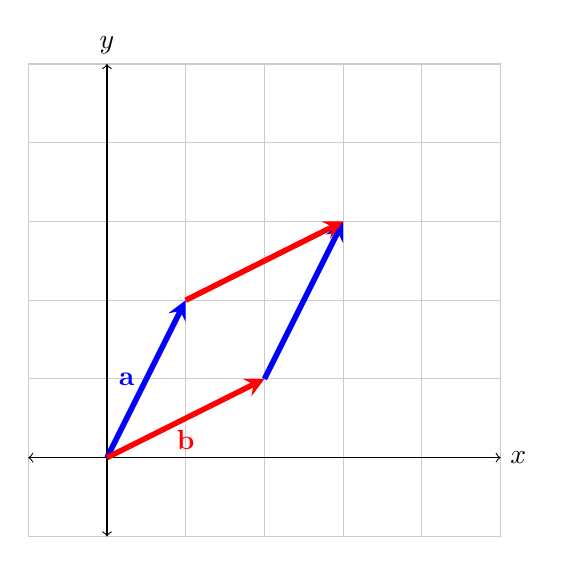
\begin{tikzpicture}
        \draw[thin,gray!40] (-1,-1) grid (5,5);
        \draw[<->] (-1,0)--(5,0) node[right]{$x$};
        \draw[<->] (0,-1)--(0,5) node[above]{$y$};
        \draw[line width=2pt,blue,-stealth](0,0)--(1,2) node[anchor=east] at (.5,1){$\mathbf{a}$};
        \draw[line width=2pt, red, -stealth](0,0)--(2,1) node[anchor=north] at (1,.5){$\mathbf{b}$};
        \draw[line width=2pt,blue,-stealth](2,1)--(3,3) node[anchor=east] at (.5,1){};
        \draw[line width=2pt, red, -stealth](1,2)--(3,3) node[anchor=north] at (1,.5){};
        \end{tikzpicture}
        \end{center}
        What is the area of this parallelogram? 
        \end{exercise}
        
        \begin{exercise}
        The area of the parallelogram defined by $\mathbf{a}=(3,1,-1)$ and $\mathbf{b}=(1,2,-3)$ can be found by computing $\|\mathbf{a}\times \mathbf{b}\|$.  Compute this.
        \end{exercise}
        
        \begin{ex}{Angular Velocity and Right-Hand Rule}{angular_velocity}
        For a particle moving along a circle with radius $r$ we can define a quantity called the \emph{angular velocity} and denote it by $\mathbf{\omega}$.  Then, for example, the time it takes for the particle to travel around the whole circle (the \emph{period}) is
        \[
        \tau = \frac{2\pi r}{\|\mathbf{\mathbf{\omega}}\|}.
        \]
        It turns out that the angular velocity of this particle at any point is given by
        \[
        \mathbf{\omega}=\frac{\mathbf{r}\times \mathbf{v}}{\|\mathbf{r}\|^2}.
        \]
        We can also find $\mathbf{v}$ from $\mathbf{\omega}$ and $\mathbf{r}$. Take a look at the figure below and note the orientation of $\mathbf{\omega}$ relative to the direction the particle travels around the circle.
        \begin{center}
        \begin{figure}[H]
            \centering
            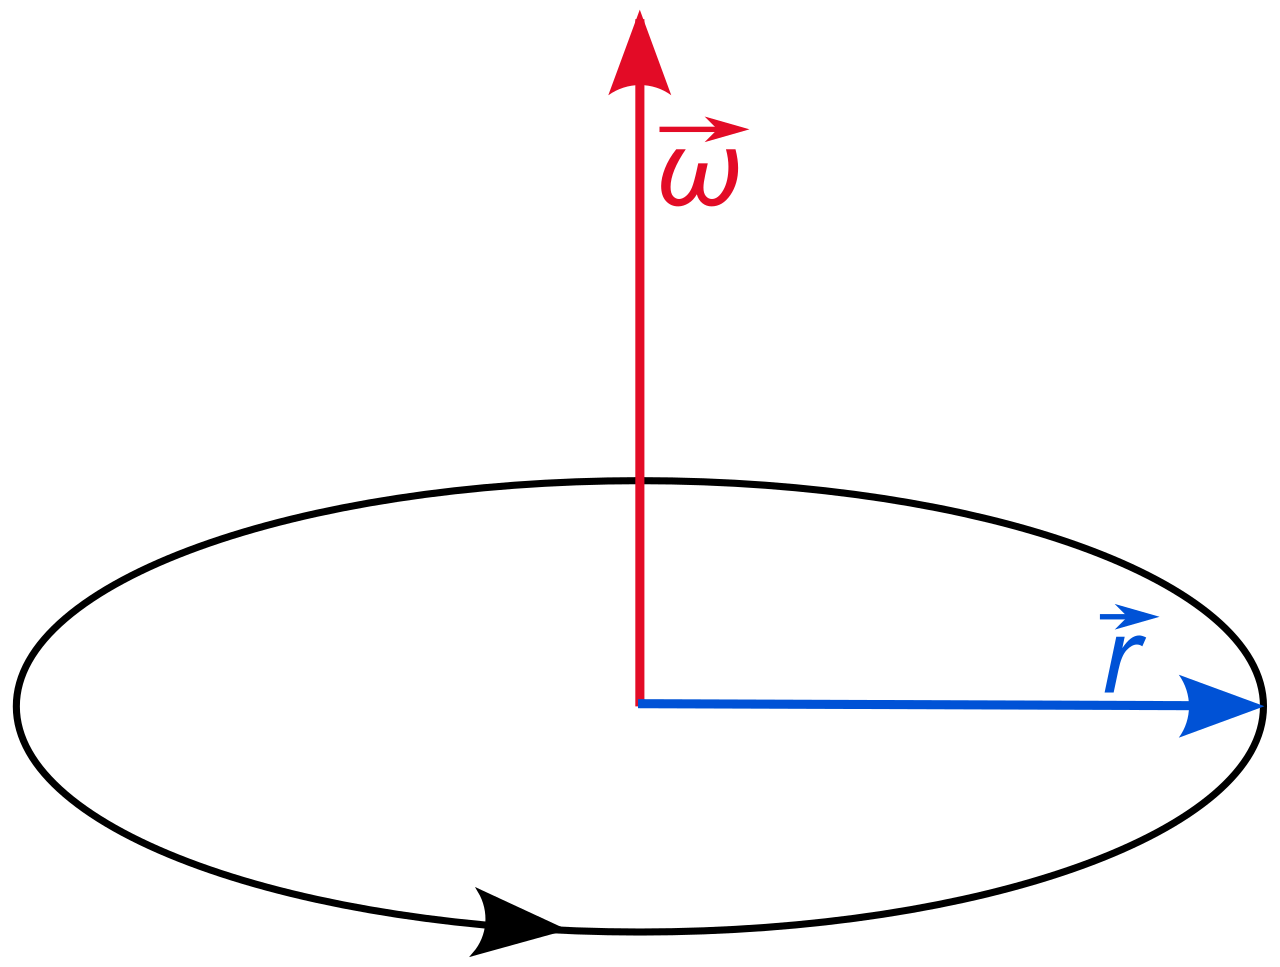
\includegraphics[width=.3\textwidth]{Figures/Angular_velocity.png}
            \caption{A particle moving around a circle of radius $\|\mathbf{r}\|$ in a counter-clockwise motion.}
            \label{angular-momentum}
        \end{figure}
        \end{center}
        Note that $\mathbf{v}$ would be tangent to this circle at the point $\mathbf{r}$ and pointing along the direction of travel.
        
        It turns out that $\mathbf{\omega}$ is a vector pointing perpendicularly to the plane that the circle the particle traverses is in. Which way does $\mathbf{\omega}$ point? We need the \emph{right-hand rule}!
        \begin{center}
        \begin{figure}[H]
            \centering
            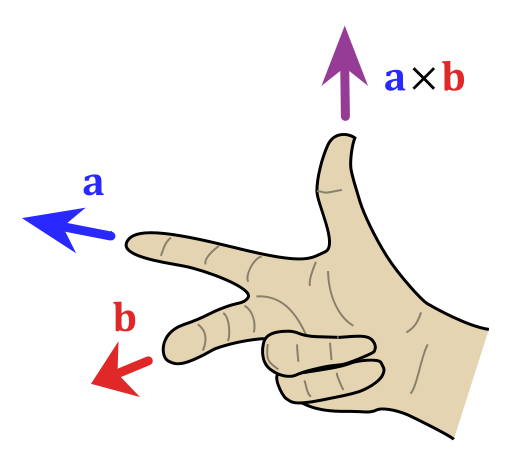
\includegraphics[width=.3\textwidth]{Figures/507px-Right_hand_rule_cross_product.png}
            \caption{The right-hand rule.}
        \end{figure}
        \end{center}
        To see how this works, we let $\mathbf{a}=\mathbf{r}$ be our index finger, then $\mathbf{v}=\mathbf{b}$ be our middle finger.  The resulting direction of $\mathbf{r}\times \mathbf{v}=\mathbf{\omega}$ is then pointing in the direction we see from Figure \ref{angular-momentum}.
        \end{ex}
        
        
    \chapter{Linear Transformations and Matrices}
        \section{Linear Transformations}
        Now that we have set the stage for vectors and the products between them, we would like to investigate how we can transform these vectors.  Specifically, we will first care about functions that are \emph{linear}.  These will be functions that stretch and rotate vectors and possibly change dimension all while leaving the origin alone.
        
        \begin{df}{Linear Transformation}{linear_transformation}
        A \textbf{linear transformation} \index{linear!transformation} is a function
        \[
        T\colon \R^n \to \R^m
        \]
        that satisfies the following requirements:
        \begin{enumerate}[(i)]
            \item $T(\mathbf{a}+\mathbf{b})=T(\mathbf{a})+T(\mathbf{b})$,
            \item $T(\lambda \mathbf{a})=\lambda T(\mathbf{a})$,
            \item $T(\mathbf{0})=\mathbf{0}$.
        \end{enumerate}
        \end{df}
        
        \begin{remark}
        These rules should seem similar to the properties of the derivative and integral.  We'll find that what we're building here will let us properly talk about derivatives in multiple dimensions.
        \end{remark}        
        
        \begin{ex}{Linear or Not?}{linear_or_not}
        Which of the following are linear transformations? Why or why not?
        \begin{enumerate}[(a)]
            \item $f\colon \R \to \R$ given by $f(x)=\lambda x$.
            \item $g\colon \R \to \R$ given by $g(x)=2x+1.$
            \item $h\colon \R \to \R$ given by $h(x)=x^2.$
            \item $T \colon \R^3 \to \R^3$ given by
            \[
            T\left( \begin{bmatrix} x\\ y\\ z \end{bmatrix} \right) = \begin{bmatrix} y\\ x\\ z \end{bmatrix}.
            \]
        \end{enumerate}
        \end{ex}
        
        \begin{ex}{Dot Product is Linear}{dot_prod_linear}
        If we choose a fixed vector $\mathbf{v}$, then the dot product of another vector $\mathbf{a}$ with $\mathbf{v}$ is itself an example of a linear transformation! It's also a good example of how the input dimension can differ from the output dimension.  Let us write $\textrm{Dot}_\mathbf{v}\colon \R^3 \to \R$ which is given by
        \[
        \textrm{Dot}_\mathbf{v}(\mathbf{a})=\mathbf{a}\cdot \mathbf{v}=a_xv_x+a_yv_y+a_zv_z.
        \]
        \end{ex}
        
        \begin{ex}{Scaling is Linear}
        Consider $T \colon \R^2 \to \R^2$ given by
        \[
        T\left( \begin{bmatrix} x\\ y \end{bmatrix}\right)
        = \begin{bmatrix} \lambda x\\ \gamma y \end{bmatrix}.
        \]
        This transformation scales the $x$-component of our vector by $\lambda$ and scales the $y$-component by $\gamma$.
        \end{ex}
        
        \begin{exercise}
        Pick a vector in the plane and draw a picture of the scaling transformation.
        \end{exercise}
        
        \begin{ex}{Rotation is Linear}
        Consider the following linear transformation $T\colon \R^2 \to \R^2$ given by
        \[
        T\left( \begin{bmatrix} x\\ y \end{bmatrix} \right)
        = \begin{bmatrix} x \cos \theta - y \sin \theta\\ x \sin \theta +y \cos \theta \end{bmatrix} = \begin{bmatrix} x'\\ y' \end{bmatrix}.
        \]
        This transformation rotates a vector by $\theta$ in the counter-clockwise direction. 
        \begin{figure}[H]
            \centering
            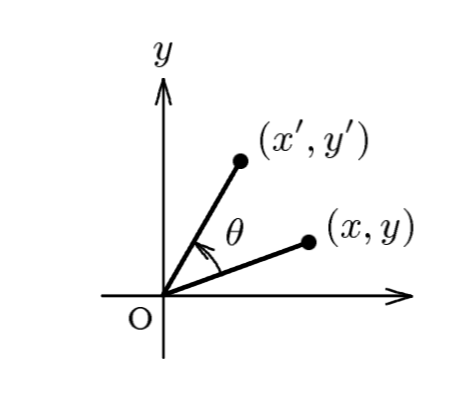
\includegraphics[width=.3\textwidth]{Figures/plane_rotation.png}
        \end{figure}
        \end{ex}
        
    \section{Matrices}
        
        The salient fact of linear transformations is how we can represent them.  As it turns out, any linear transformation $T\colon \R^n \to \R^m$ can be written like:
        \[
        T\left( \begin{bmatrix} x_1 \\ x_2 \\ \vdots \\ x_n \end{bmatrix}\right)
        = \begin{bmatrix} y_1 \\ y_2 \\ \vdots \\ y_m \end{bmatrix},
        \]
        where 
        \begin{align*}
            y_1 &= a_{11} x_1 + a_{12} x_2 + a_{13} x_3 + \cdots + a_{1n} x_n\\
            y_2 &= a_{21} x_1 + a_{22} x_2 + a_{23} x_3 + \cdots + a_{2n} x_n\\
            y_3 &= a_{31} x_1 + a_{32} x_2 + a_{33} x_3 + \cdots + a_{3n} x_n\\
            \vdots\\
            y_m &= a_{m1} x_1 + a_{m2} x_2 + a_{m3} x_3 + \cdots + a_{mn} x_n.
        \end{align*}
        The linear transformation is captured entirely by the \emph{matrix} of numbers
        \[
        \begin{bmatrix}
        a_{11} & a_{12} & a_{13} & \cdots & a_{1n}\\
        a_{21} & a_{22} & a_{23} & \cdots & a_{2n}\\
        a_{31} & a_{32} & a_{33} & \cdots & a_{3n}\\
        \vdots & \vdots & \vdots & & \vdots \\
        a_{n1} & a_{n2} & a_{n3} & \cdots & a_{nm}
        \end{bmatrix}
        \]
        
        We've seen that matrices are the fundamental object we need to describe linear transformations.  They aren't necessary to use, but they make computation and understanding a bit easier.  It turns out that we can also think of vectors as special cases of matrices, which makes the idea of studying matrices themselves all that much better. 
        
        \section{Matrix Algebra}
        Just as we did with vectors, we want to understand what we can do with these matrices algebraically.  
        
        We will call a matrix with $n$-rows and $m$-columns an \textbf{$n\times m$-matrix} (read: $n$ by $m$ matrix).  These take the form:
        \[\mathbf{A}=
        \begin{bmatrix}
        a_{11} & a_{12} & a_{13} & \cdots & a_{1n}\\
        a_{21} & a_{22} & a_{23} & \cdots & a_{2n}\\
        a_{31} & a_{32} & a_{33} & \cdots & a_{3n}\\
        \vdots & \vdots & \vdots & & \vdots \\
        a_{n1} & a_{n2} & a_{n3} & \cdots & a_{nm}
        \end{bmatrix}.
        \]
        We use a capital boldfaced letter to denote a matrix. Each entry of the matrix will be given by a lowercase letter with subscripts $a_{ij}$.  The subscripts will tell you which row and column the entry is located. For example, $a_{25}$ would be the entry in the 2$^\textrm{nd}$ row and $5^\textrm{th}$ column.
        
        \begin{enumerate}[(i)]
            \item \textbf{Equality:} Matrices are equal if each entry is equal. That is, given $\mathbf{A}$ and $\mathbf{B}$, we say $\mathbf{A}=\mathbf{B}$ if $a_{ij}=b_{ij}$ for each pair $i,j$.  Clearly if these matrices are not the same ``shape" (meaning, they have a different number of rows or columns), then they cannot be the same.  Just as a 2-dimensional vector cannot be the same as a 3-dimensional one.  They are distinctly different objects.
            
            \item \textbf{Addition:} We can add matrices of the same shape.  We write $\mathbf{A}+\mathbf{B}=\mathbf{C}$ and create the new matrix $\mathbf{C}$ by adding the entries.  That is, $c_{ij}=a_{ij}+b_{ij}$.  
            
            \item \textbf{Scalar Multiplication:} We can also scale matrices.  We do this by scaling the entries.  So, if we have $\lambda \mathbf{A}=\mathbf{B}$, then we know the entries of $\mathbf{B}$ are given by $b_{ij}=\lambda a_{ij}$.
            
            \item \textbf{Matrix Multiplication:} It is also possible to multiply two matrices together.  Recall that matrices are how we capture the information of a linear transformation. Matrix multiplication will capture the idea of composing two linear transformations. 
            
            We can multiply matrices $\mathbf{A}$ and $\mathbf{B}$ if 
            \[
            \textrm{the number of columns of $\mathbf{A}$}=\textrm{the number of rows of $\mathbf{B}$}.
            \]
            If $\mathbf{A}$ is an $n\times m$-matrix and $\mathbf{B}$ is an $m\times p$-matrix, then $\mathbf{C}=\mathbf{AB}$ is an $n\times p$ matrix.  You can remember this helpful fact:
            \[
            (n\times \underbrace{m)\cdot (m}_{\textrm{the same}}\times p)
            \]
            and
            \[
            (\underbrace{n}\times m)\cdot (m\times \underbrace{p})
            \]      
            gives the dimensions of the resulting matrix.
            
            How we perform this matrix multiplication looks a bit ugly at first, but it ends up being slightly easier after digesting this a bit. We have that the components of $\mathbf{C}=\mathbf{AB}$ are
            \[
            c_{ij}=\sum_{k=1}^m a_{ik}b_{kj}.
            \]
            
            Let us take the example of an $1\times n$-matrix $\mathbf{A}$ and a $n\times 1$-matrix $\mathbf{B}$. Then
            \[
            \mathbf{AB}=
            \begin{bmatrix} a_1 & a_2 & \cdots & a_n\end{bmatrix}
            \begin{bmatrix} b_1\\ b_2 \\ \vdots \\ b_n\end{bmatrix}=a_1b_1+b_2b_2+\cdots+a_nb_n=\sum_{k=1}^n a_kb_k.
            \]
            This is the dot product of two vectors!  As it turns out, we can decompose matrix multiplication into a bunch of dot products. 
            
            In general, the $i$th row of a matrix $\mathbf{A}$ is a vector with $m$ elements, the $j$th column of a matrix $\mathbf{B}$ is a vector with $m$ elements, and the dot product of these two vectors gives the entry $c_{ij}$ of the matrix $\mathbf{AB}=\mathbf{C}$.
            
            \begin{remark}
            This all means it is possible to take linear combinations of matrices as well!
            \end{remark}
            
            \begin{ex}{Multiplying Matrices}{multiplying_matrices}
            Let us multiply the following matrices:
            \[
            \mathbf{A}=\begin{bmatrix} 2 & 0 & -3\\ 1&1&-2\end{bmatrix} \quad \mathbf{B}=\begin{bmatrix} 2&3&4&1\\1&2&2&0\\0&-1&2&0\end{bmatrix}.
            \]
            Verify that you get
            \[
            \mathbf{AB}=\begin{bmatrix} 4&9&2&2\\3&7&2&1\end{bmatrix}.
            \]
            \end{ex}
            
            
            \subsubsection{Properties of Matrix Multiplication}
            
            Matrices will behave in the following ways:
            \begin{enumerate}[(i)]
                \item \textbf{Associativity:} The order in which you choose to multiply matrices does not matter.  That is 
                \[\mathbf{A}(\mathbf{BC})=(\mathbf{AB})\mathbf{C}=\mathbf{ABC}.\]
                \item \textbf{Distributivity:} We can multiply matrices over sums. That is
                \[
                \mathbf{A}(\mathbf{B}+\mathbf{C})=\mathbf{AB}+\mathbf{AC}.
                \]
                \item \textbf{(non)-Commutivity:} In general, we have
                \[
                \mathbf{AB}\neq \mathbf{BA}.
                \]
                However, there are certain types of matrices that do commute with each other.
            \end{enumerate}
            
            
        \end{enumerate}
        
        Right now we have the ability to write linear transformations as matrices.  We can also multiply these matrices.  Keep in mind that this in some way mimics composing functions.
        
    \section{The Determinant}
        We now want to understand further properties of matrices.  One important one is the \textbf{determinant.} The determinant is a special number associated to only $n\times n$-matrices.  We often call these matrices \emph{square}.  More on this later.  
        
        We can collect vectors $\mathbf{v}_1,\dots,\mathbf{v}_n$ into a matrix by placing each vector in a column of its own.  That is
        \[
        A=\begin{bmatrix}
        \mathbf{v}_1 &\mathbf{v}_2 &\cdots &\mathbf{v}_n
        \end{bmatrix}.
        \]
        If these are $n$-dimensional vectors, then this matrix is square.  Then the determinant of this matrix is written $\det(A)$. Let's now stick with just $2$ and $3$-dimensions as this will be all we need.
        
        \begin{example}[Area of a parallelogram]
        Say we have the vectors
        \[
        \mathbf{a}=\begin{bmatrix} 2\\ 0 \end{bmatrix} \quad \mathbf{b}=
        \begin{bmatrix} 1\\ 3 \end{bmatrix}.
        \]
        What is the area of the parallelogram that these vectors create? (See previous notes for how the cross product can do this.  We'll see that the cross product is highly related to determinants.)
        
        \begin{center}
        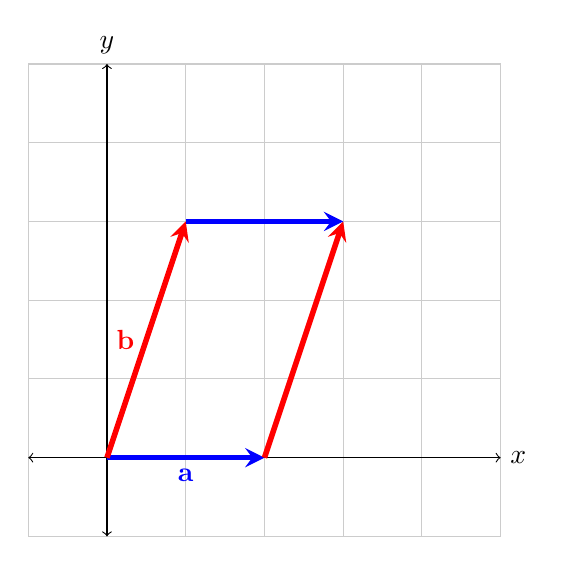
\begin{tikzpicture}
        \draw[thin,gray!40] (-1,-1) grid (5,5);
        \draw[<->] (-1,0)--(5,0) node[right]{$x$};
        \draw[<->] (0,-1)--(0,5) node[above]{$y$};
        \draw[line width=2pt,blue,-stealth](0,0)--(2,0) node[anchor=north] at (1,0){$\mathbf{a}$};
        \draw[line width=2pt, red, -stealth](0,0)--(1,3) node[anchor=east] at (.5,1.5){$\mathbf{b}$};
        \draw[line width=2pt,red,-stealth](2,0)--(3,3) node[anchor=east] at (.5,1){};
        \draw[line width=2pt, blue, -stealth](1,3)--(3,3) node[anchor=north] at (1,.5){};
        \end{tikzpicture}
        \end{center}
        The trick to finding the area here is to take move a triangle and fill in a gap. We do this like so:
        \begin{center}
        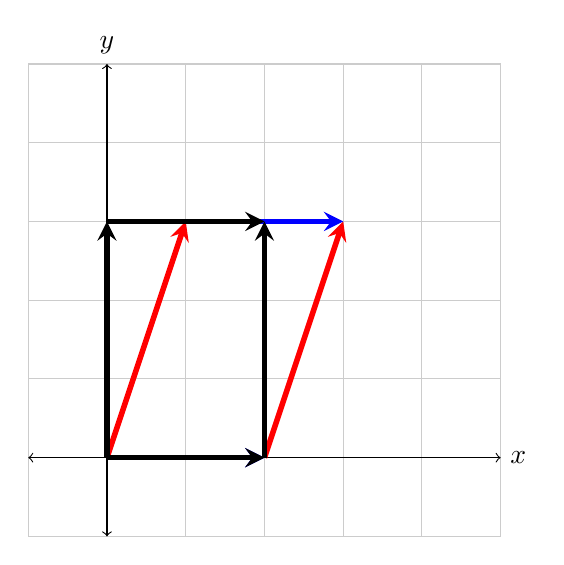
\begin{tikzpicture}
        \draw[thin,gray!40] (-1,-1) grid (5,5);
        \draw[<->] (-1,0)--(5,0) node[right]{$x$};
        \draw[<->] (0,-1)--(0,5) node[above]{$y$};
        \draw[line width=2pt,blue,-stealth](0,0)--(2,0) node[anchor=north] at (1,0){};
        \draw[line width=2pt, red, -stealth](0,0)--(1,3) node[anchor=east] at (.5,1.5){};
        \draw[line width=2pt,red,-stealth](2,0)--(3,3) node[anchor=east] at (.5,1){};
        \draw[line width=2pt, blue, -stealth](1,3)--(3,3) node[anchor=north] at (1,.5){};
        \draw[line width=2pt, black, -stealth](2,0)--(2,3) node[anchor=north] at (1,.5){};    
        \draw[line width=2pt, black, -stealth](0,0)--(0,3) node[anchor=north] at (1,.5){};
        \draw[line width=2pt, black, -stealth](0,0)--(2,0) node[anchor=north] at (1,.5){};
        \draw[line width=2pt, black, -stealth](0,3)--(2,3) node[anchor=north] at (1,.5){};
        \end{tikzpicture}
        \end{center}
        In the above, we've moved a triangle from the right, to the left, to make the black rectangle.  This rectangle then has an area of $2\cdot 3=6.$
        
        Let us see the way we can do this that does not require this extra work.  Let us place these vectors into a matrix:
        \[
        A=\begin{bmatrix} \mathbf{a} & \mathbf{b} \end{bmatrix}=
        \begin{bmatrix} 2 & 1\\ 0 & 3 \end{bmatrix}.
        \]
        Then $\det(A)$ will give us the area of this parallelogram! We have
        \[
        \det(A)=2\cdot 3 - 1\cdot 0 = 6.
        \]
        This begs the question, what is this formula in general?
        \end{example}
        
        To compute the determinant of a $2\times 2$-matrix
        \[
        A=\begin{bmatrix} a & b\\ c & d \end{bmatrix},
        \]
        we have
        \[
        \det(A) = ad-bc.
        \]
        You can remember this by thinking that you multiply top left with bottom right, then subtract the product of top right with bottom left.  
        \begin{ex}{Volume of a parallelopiped}{volume_of_parallelopiped}
        We often want to find volumes of parallelogram shaped higher dimensional objects.  In general, we call these \emph{parallelopipeds}.  
        
        For example, in $3$-dimensional space, we can take three vectors
        \[
        \mathbf{a}=\begin{bmatrix} 0 & 1 & 0 \end{bmatrix}\quad
        \mathbf{b}=\begin{bmatrix} 1 & 0 & 0 \end{bmatrix}\quad
        \mathbf{c}=\begin{bmatrix} 0 & 0 & 2 \end{bmatrix}.
        \]
        These, when combined properly, enclose a volume of a parallelopiped. 
\begin{center}
\tdplotsetmaincoords{60}{120} 
\begin{tikzpicture} [scale=3, tdplot_main_coords, axis/.style={->,black,thick}, 
vector/.style={-stealth,blue,very thick}, 
vector guide/.style={dashed,red,thick}]

%standard tikz coordinate definition using x, y, z coords
\coordinate (O) at (0,0,0);

%tikz-3dplot coordinate definition using x, y, z coords

\pgfmathsetmacro{\ax}{0.6}
\pgfmathsetmacro{\ay}{1}
\pgfmathsetmacro{\az}{0.8}

\coordinate (P) at (\ax,\ay,\az);

%draw axes
\draw[axis] (0,0,0) -- (1,0,0) node[anchor=north east]{$x$};
\draw[axis] (0,0,0) -- (0,1,0) node[anchor=north west]{$y$};
\draw[axis] (0,0,0) -- (0,0,1) node[anchor=south]{$z$};


\draw[line width=2pt, red, -stealth](0,0,0)--(0,3/4,0) node[anchor=north west] at (0,3/4,0){$\mathbf{a}$};
\draw[line width=2pt, blue, -stealth](0,0,0)--(1/4,0,0) node[anchor=north] at (1/4,0,0){$\mathbf{b}$};
\draw[line width=2pt, green, -stealth](0,0,0)--(0,0,1/2) node[anchor=east] at (0,0,1/2){$\mathbf{c}$};

\end{tikzpicture}
\end{center}
\begin{center}
\tdplotsetmaincoords{60}{120} 
\begin{tikzpicture} [scale=3, tdplot_main_coords, axis/.style={->,black,thick}, 
vector/.style={-stealth,blue,very thick}, 
vector guide/.style={dashed,red,thick}]

%standard tikz coordinate definition using x, y, z coords
\coordinate (O) at (0,0,0);

%tikz-3dplot coordinate definition using x, y, z coords

\pgfmathsetmacro{\ax}{0.6}
\pgfmathsetmacro{\ay}{1}
\pgfmathsetmacro{\az}{0.8}

\coordinate (P) at (\ax,\ay,\az);

%draw axes
\draw[axis] (0,0,0) -- (1,0,0) node[anchor=north east]{$x$};
\draw[axis] (0,0,0) -- (0,1,0) node[anchor=north west]{$y$};
\draw[axis] (0,0,0) -- (0,0,1) node[anchor=south]{$z$};


\draw[line width=2pt, red, -stealth](0,0,0)--(0,3/4,0) node[anchor=north west] at (0,1,0){};
\draw[line width=2pt, blue, -stealth](0,0,0)--(1/3,0,0) node[anchor=north] at (1/3,0,0){};
\draw[line width=2pt, green, -stealth](0,0,0)--(0,0,1/2) node[anchor=east] at (0,0,2/3){};

\draw[line width=2pt, red, -stealth](1/4,0,0)--(1/4,3/4,0) node[anchor=north west] at (1/3,2/3,3/3){};
\draw[line width=2pt, blue, -stealth](0,3/4,0)--(1/4,3/4,0) node[anchor=north] at (1/3,0,0){};
\draw[line width=2pt, green, -stealth](1/4,0,0)--(1/4,0,1/2) node[anchor=east] at (0,0,2/3){};

\draw[line width=2pt, red, -stealth](1/4,0,1/2)--(1/4,3/4,1/2) node[anchor=north west] at (1/3,2/3,3/3){};
\draw[line width=2pt, blue, -stealth](0,0,1/2)--(1/4,0,1/2) node[anchor=north] at (1/3,0,0){};
\draw[line width=2pt, green, -stealth](0,3/4,0)--(0,3/4,1/2) node[anchor=east] at (0,0,2/3){};

\draw[line width=2pt, red, -stealth](0,0,1/2)--(0,3/4,1/2) node[anchor=north west] at (1/3,2/3,3/3){};
\draw[line width=2pt, blue, -stealth](0,3/4,1/2)--(1/4,3/4,1/2) node[anchor=north] at (1/3,0,0){};
\draw[line width=2pt, green, -stealth](1/4,3/4,0)--(1/4,3/4,1/2) node[anchor=east] at (0,0,2/3){};
\end{tikzpicture}
\end{center}
Of course, I picked an easy example for the illustration.  But what is the volume? Here we again know we can compute this the usual way and we get that the volume is $1\cdot 1 \cdot 2 = 2.$

If we arrange these vectors in a matrix
\[
A=\begin{bmatrix} \mathbf{a} & \mathbf{b} &\mathbf{c} \end{bmatrix} =
\begin{bmatrix} 0 & 1 & 0 \\ 1 & 0 & 0 \\ 0 & 0 & 2 \end{bmatrix},
\]
we want $\det(A)$ to reflect this volume. It turns out the way we compute $\det(A)$ comes from using the determinant of $2\times 2$-matrices.  Let me explain further.

Let me write this matrix as a tool:
\[
\begin{bmatrix} + & - & +\\ - & + & - \\ + & - & + \end{bmatrix}.
\]
What we will use this for is a memory tool when we do something called the \emph{cofactor expansion}.  What I will do is choose a row of column to \emph{expand} across.  Let me choose the top row for simplicity's sake.  The top row will have signs $+-+$ that will show up in our computation. We will also have to take into account the element in the original matrix and multiply by that.

We start with the top left of $A$ and we will have a $+$ sign.  The top left of $A$ is element $a_{11}$ and so we remove the $1^{\textrm{st}}$ row and column from $A$ to give
\[
\textrm{Cof}_{11}(A)=\begin{bmatrix} 0 & 0 \\ 0 & 2 \end{bmatrix}.
\]
Then $\det(\textrm{Cof}_{11})(A))=0\cdot 2 - 0 \cdot 0=0.$

We now move on to the top middle of $A$ and will have a $-$ sign. The top middle element is $a_{12}$ and so we remove the $1^{\textrm{st}}$ row and $2^{\textrm{nd}}$ column of $A$ to give
\[
\textrm{Cof}_{12}(A)=\begin{bmatrix} 1 & 0 \\ 0 & 2\end{bmatrix}.
\]
Then $\det(\textrm{Cof}_{12}(A))=1\cdot 2-0 \cdot 0=2.$

Lastly, we move on to the top right of $A$ and will have a $+$ sign. The top right element is $a_{13}$ and so we remove the $1^{\textrm{st}}$ row and $3^{\textrm{rd}}$ column of $A$ to give
\[
\textrm{Cof}_{13}(A)=\begin{bmatrix} 1 & 0 \\ 0 & 0\end{bmatrix}.
\]
Then $\det(\textrm{Cof}_{12}(A))=1\cdot 0-0 \cdot 0=0.$

So $\det(A)=+(0)\cdot\det(\textrm{Cof}_{11}(A))-(1)\cdot\det(\textrm{Cof}_{12}(A))+(0)\cdot\det(\textrm{Cof}_{13}(A))=-2.$ So what we got was a negative of our predicted volume.
        \end{ex}

        \begin{exercise} Let
        \[
        A=\begin{bmatrix} 1 & 2 & 3 \\ 4 & 5 & 6 \\ 7 & 8 & 9 \end{bmatrix}.
        \]
        \begin{enumerate}[(a)]
            \item Find $\textrm{Cof}_{11}(A)$.
            \item Find $\textrm{Cof}_{22}(A)$.
            \item Find $\textrm{Cof}_{23}(A)$.
            \item Compute $\det(A)$.
        \end{enumerate}
        
        \end{exercise}
        
        \begin{question}
        What does it mean if $\det(A)=0$ for some matrix $A$?
        \end{question}
        
        \begin{answer}
        It means that we have a parallelopiped with zero volume.  Which means our three vectors actually lie in a plane, or even on a single line.  This is an important fact that will come up when we solve systems of equations!
        \end{answer}
        
        \begin{remark}
        Determinants can be computed in arbitrary dimension using the same process above.  It get's rather annoying and I do not find it necessary for us.
        \end{remark}
        
        \begin{remark}
        The sign of a determinant being negative has to do with an ``orientation" of the volume.  We like to choose ``right-handed" coordinates and its possible that the matrix, in a sense, can give us ``left-handed" coordinates.  This gives us a negative volume.
        \end{remark}
        
        \begin{ex}{Cross product from the Determinant}{cross_prod_det}
        You can compute the cross product from the determinant.  (You should be warned: this is an abuse of notation and a somewhat weird coincidence.) Let us create choose two vectors $\mathbf{v}$ and $\mathbf{w}$. We place them in a matrix $A$ as follows:
        \[
        A=
        \begin{bmatrix}
        \mathbf{\hat{\i}} & \mathbf{\hat{\j}} & \mathbf{\hat{k}}\\
        v_x & v_y & v_z\\
        w_x & w_y & w_z
        \end{bmatrix}.
        \]
        Then $\det(A)$ will give us the cross product $\mathbf{v}\times \mathbf{w}$.  Just know that you are briefly ignoring the fact that $\mathbf{\hat{\i}}$, $\mathbf{\hat{\j}}$, $\mathbf{\hat{k}}$ are actually vectors when you compute this.  Treat them as numbers until you get your final result.
        \end{ex}
        
        \begin{ex}{Determinant of a $3\times 3$-Matrix}{det_of_3x3}
        Let us write
        \[
        A=\begin{bmatrix} a_{11} & a_{12} & a_{13} \\ a_{21} & a_{22} & a_{23}\\ a_{31} & a_{32} & a_{33} \end{bmatrix}.
        \]
        We can expand across the first row and get
        \[
        \det(A)=a_{11}\cdot \det(\textrm{Cof}_{11}(A)) - a_{12}\cdot \det(\textrm{Cof}_{12}(A))+ a_{13}\cdot \det(\textrm{Cof}_{13}(A)).
        \]
        \end{ex}
        
        \begin{exercise}
        How could you write the determinant of a $3x3$-matrix $A$ that we expand along the second column?
        \end{exercise}
        
        \subsubsection{Properties of determinants}
        There are a few nice properties of determinants to keep in mind. 
        \begin{enumerate}[(i)]
            \item \textbf{Transposition:} If we exchange rows for columns in a matrix (that is, to take the \emph{transpose matrix}, then the value of the determinant is the same. Given
            \[
            A=\begin{bmatrix}
            a_{11} & a_{12} & a_{13}\\
            a_{21} & a_{22} & a_{23}\\
            a_{31} & a_{32} & a_{33}
            \end{bmatrix}
            \]
            we write the transpose matrix
            \[
            A^T=\begin{bmatrix}
            a_{11} & a_{21} & a_{31}\\
            a_{12} & a_{22} & a_{32}\\
            a_{13} & a_{23} & a_{33}
            \end{bmatrix}.
            \]
            So $a_{ij}\mapsto a_{ji}$. Then
            \[
            \det(A)=\det(A^T).
            \]
            
            \item \textbf{Multiplication by constants:} If we multiply a row or column by a scalar, then the determinant is also multiplied by that scalar.  So we have
            \[
            A_\lambda=\begin{bmatrix}
            \lambda a_{11} & \lambda a_{12} & \lambda a_{13}\\
            a_{21} & a_{22} & a_{23}\\
            a_{31} & a_{32} & a_{33}
            \end{bmatrix}
            \]
            Then
            \[
            \det(A_\lambda)=\lambda \det(A).
            \]
            
            \item \textbf{Addition of rows or columns:} If  we add to any row or column, then we can sum the determinants.  So we have
            \[
            \left| \begin{array}{ccc}
                a_{11} + v_1 & a_{12} & a_{13} \\
                a_{21} + v_2 & a_{22} & a_{23} \\
                a_{31} + v_3 & a_{32} & a_{33}
            \end{array}\right|=\left| \begin{array}{ccc}
                a_{11} & a_{12} & a_{13} \\
                a_{21} & a_{22} & a_{23} \\
                a_{31} & a_{32} & a_{33}
            \end{array}\right|+\left| \begin{array}{ccc}
                v_1 & a_{12} & a_{13} \\
                v_2 & a_{22} & a_{23} \\
                v_3 & a_{32} & a_{33}
            \end{array}\right|
            \]
            
            \item \textbf{Exchanging rows or columns:} If we swap rows or columns, the determinant is multiplied by $-1$. So we have
            \[
            \left|\begin{array}{ccc}
                a_{11} & a_{12} & a_{13} \\
                a_{21} & a_{22} & a_{23} \\
                a_{31} & a_{32} & a_{33}
            \end{array}\right|=-
            \left|\begin{array}{ccc}
                a_{12} & a_{11} & a_{13} \\
                a_{22} & a_{21} & a_{23} \\
                a_{32} & a_{31} & a_{33}
            \end{array}\right|
            \]
            
            \item \textbf{Linearly-dependent rows or columns:} If a column (resp. row) of a matrix can be written as a linear combination of the other two columns (resp. rows), then the determinant is zero.  This is basically saying that all three vectors lie in a single plane and so the volume of the parallelopiped given by the three vectors (as columns in the matrix) create no volume.
            
            Say we can write
            \begin{align*}
                a_{11}&=\lambda a_{12} + \mu a_{13}\\
                a_{21}&=\lambda a_{22} + \mu a_{23}\\
                a_{31}&=\lambda a_{32} + \mu a_{33}.
            \end{align*}
            Then $\det(A)=0.$
        \end{enumerate}
        
        These qualities of the determinant will give us the ability to analyze the next subsection properly.
        
        
        \section{Systems of Linear Equations}
        Often times we wish to solve equations of the form:
        \[
        A\mathbf{x}=\mathbf{b}
        \]
        where $A$ is an $n\times m$-matrix, $\mathbf{x}$ is an $m$-dimensional vector, and $\mathbf{b}$ is an $n$-dimensional vector.  Let us write out what this looks like:
        \[
        \begin{bmatrix}
        a_{11} & a_{12} & \cdots & a_{1m}\\
        a_{21} & a_{22} & \cdots & a_{2m}\\
        \vdots & \vdots & \cdots & \vdots\\
        a_{n1} & a_{n2} & \cdots & a_{nm}
        \end{bmatrix}
        \begin{bmatrix}
        x_1\\ x_2 \\ \vdots \\ x_m
        \end{bmatrix}
        =\begin{bmatrix}
        b_1 \\ b_2 \\ \vdots \\ b_n
        \end{bmatrix},
        \]
        gives us a set of equations
        \begin{align*}
        a_{11} x_1 + a_{12}x_2 + \cdots a_{1m} x_m &= b_1\\
        a_{21} x_1 + a_{22} x_2 + \cdots a_{2m} x_m &= b_2
        &\vdots\\
        a_{n1} x_1 + a_{n2} x_2 + \cdots a_{nm} x_m &= b_n.
        \end{align*}
        We call these equations a \textbf{system of linear equations}.
        
        In general, if $n\neq m$, the methods of solving are exactly what we will cover aside from the ability to use the determinant.  However, there are some subtle issues with the $n\neq m$ case that I won't go into detail on.  If you're interested, look up \emph{over} and \emph{underdetermined} systems. From this point on we will assume $A$ to be $n\times n$.
        
        \subsubsection{Homogeneous Equations}
        Let us begin with the easiest case to analyze, the \textbf{homogeneous equations}. These take the form 
        \[
        A\mathbf{x}=\mathbf{0}.
        \]
        This yields the equations:
        \begin{align*}
            a_{11}x_1 + a_{12}x_2 + \cdots + a_{1n}x_n &=0\\
            a_{21}x_1 + a_{22} x_2 + \cdots + a_{2n}x_n &=0\\
            &\vdots\\
            a_{n1}x_1 +a_{n2}+ \cdots +a_{nn}x_n &=0.
        \end{align*}
        
        \begin{prop}{Solutions to Homogeneous Equations}{solutions_to_homo}
        The homogeneous equations have solutions:
        \begin{itemize}
            \item (Trivial) $\mathbf{x}=\mathbf{0}$ if and only if $\det(A)\neq 0$;
            \item $\mathbf{x}\neq \mathbf{0}$ if and only if $\det(A)= 0$.
        \end{itemize}
        \end{prop}
        
        \begin{exercise}
        Take the determinant and then attempt to solve the following homogeneous equations.
        \begin{enumerate}[(a)]
            \item Let 
            \[
            A=\begin{bmatrix}
            1 & 1 & 0\\
            1 & 0 & 5\\
            0 & 1 & 2
            \end{bmatrix}
            \]
            and solve $A\mathbf{x}=\mathbf{0}.$
            \item Let
            \[
            B=\begin{bmatrix}
            2 & 3 & 1\\
            1 & 4 & 3\\
            1 & 2 & 1
            \end{bmatrix}
            \]
            and solve $B\mathbf{x}=\mathbf{0}.$
        \end{enumerate}
        \end{exercise}
        
        \begin{remark}
        Notice that in (b), if we add column one to column three for the matrix $B$, that we end up with column two.  This means if we treat the columns of $B$ as vectors; that is, we let
        \[
        \mathbf{v}_1=\begin{bmatrix}
        2 \\ 1 \\ 1
        \end{bmatrix} \quad 
        \mathbf{v}_2= \begin{bmatrix} 3 \\ 4 \\ 2 \end{bmatrix} \quad
        \mathbf{v}_3= \begin{bmatrix} 1 \\ 3 \\ 1 \end{bmatrix}.
        \]
        Then $\mathbf{v}_2=\mathbf{v}_1+\mathbf{v}_3$.  This means all these vectors lie in a plane, and the determinant of $B$ should be zero based on our intuition.  It also means we can solve
        \[
        \lambda_1 \mathbf{v}_1 + \lambda_2 \mathbf{v}_2 + \lambda_3 \mathbf{v}_3 = \mathbf{0}
        \]
        where $\lambda_1$, $\lambda_2$, and $\lambda_3$ are not all zero.
        
        This is a very important realization in the realm of linear systems.  With our limited time and scope, we cannot possibly do everything here.  But, keep this in mind.  There is a strong relationship between the geometry of the set of solutions and the algebra of vectors and matrices.  If this seems interesting to you, consider taking Math 369.
        \end{remark}
        
        \section{Solving Linear Systems of Equations}
        Say we are handed a matrix $A$ and an output vector $\mathbf{b}$ and we are asked to solve
        \[
        A\mathbf{x}=\mathbf{b}
        \]
        for the vector $\mathbf{x}$. If $\mathbf{b}$ is nonzero, then we call this an \textbf{inhomogeneous} linear system. If $A$ is a square matrix, we can say more.
        
        \begin{prop}{Solutions to Inhomogeneous Equations}{solutions_to_inhomo}
        The inhomogenous equations have solutions:
        \begin{itemize}
            \item A unique solution if and only if $\det(A)\neq 0$;
            \item None or possibly infinitely many solutions if $\det(A)=0$.
        \end{itemize}
        \end{prop}
        
        This proposition should feel remniscent of the case for functions $f\colon \R\to \R$.  In this case, we may have been handed a function $f$, a $y$ (output) value, and were asked to find what input $x$ corresponds to that $y$ value. That is, we want
        \[
        f(x)=y.
        \]
        Here we could sometimes find an inverse function $f^{-1}$ that would satisfy
        \[
        f^{-1}(y)=x.
        \]
        However, for example, if we had the function $f(x)=x^2$, then there was no inverse function.  Why? Well, say we let $y=1$, then $x=\pm 1$ are both solutions. More on inverses later.  
        
        For now we need a method to solve the equation $A\mathbf{x}=\mathbf{b}$ for $\mathbf{x}$. 
        
        \begin{df}{Row Operations}{row_operations}
        We call the following list of operations the \textbf{elementary row operations}.
        \begin{itemize}
            \item \textbf{Row scaling:} We can scale the rows of a matrix by any scalar value $\lambda$.
            \item \textbf{Row addition:} We can add scalar multiples of any rows to another row.
            \item \textbf{Row swapping:} We can swap any two rows.
        \end{itemize}
        These operations are elementary in the sense that they do not change the ``character" of the determinant.  This means that these will not affect the solution to our system as it will not spontaneously make a determinant change from nonzero to zero or vice-versa.  
        \end{df}
        
        \begin{df}{Augmented Matrix}{augmented_matrix}
        Given an equation $A\mathbf{x}=\mathbf{b}$, we have the \textbf{augmented matrix} \index{augmented matrix} $M$
        \[
        M=\left[\begin{array}{ccc|c}
        a_{11} & a_{12} & a_{13}  &  b_1 \\
        a_{21} & a_{22} & a_{23} & b_2\\
        a_{31} & a_{32} & a_{33} & b_3
        \end{array}\right]
        \]
        (Of course, this is just for the $3\times 3$-case.  It looks similar for the $n\times n$-case.)
        \end{df}
        
        Our goal here is to use elementary row operations to reduce our augmented matrix to the following \textbf{row echelon form}.  This will look like:
        \[
        M=\left[\begin{array}{ccc|c}
        m_{11} & m_{12} & m_{13}  &  c_1 \\
        0 & m_{22} & a_{23} & c_2\\
        0 & 0 & m_{33} & c_3
        \end{array}\right]
        \]
        where the $m_{ij}$ and $c_k$ are all (possibly) new entries since we have performed elementary row operations.  It can also be that, for example, $m_{33}$ is also zero. This will be important. This is all a bit nebulous. Let us do an example. 
        
        \begin{ex}{A System of Inhomogeneous Equations}{system_of_inhomo}
        Let us consider the following matrix equation:
        \[
        \begin{bmatrix}
        1 & 0 & 2\\
        2 & 2 & 3\\
        4 & 4 & 1
        \end{bmatrix}
        \begin{bmatrix}
        x\\
        y\\
        z
        \end{bmatrix}
        =\begin{bmatrix}
        1\\
        1\\
        1
        \end{bmatrix}.
        \]
        This gives us the following system of linear equations:
        \begin{align*}
            1x+0y+2z&=1\\
            2x+2y+3z&=1\\
            4x+4y+1z&=1.
        \end{align*}
        You can solve this by hand, but it is tedious.  We will use the row reduction technique instead.  Let us create the augmented matrix
        \[
        \left[\begin{array}{ccc|c}
        1 & 0 & 2 & 1 \\
        2 & 2 & 3 & 1 \\
        4 & 4 & 1 & 1
        \end{array}\right].
        \]
        We can then do row operations to get our result
        \[
        \left[\begin{array}{ccc|c}
        1 & 0 & 2 & 1 \\
        2 & 2 & 3 & 1 \\
        4 & 4 & 1 & 1
        \end{array}\right] \underrightarrow{-2 R_2 \textrm{ from } R_3} 
        \left[\begin{array}{ccc|c}
        1 & 0 & 2 & 1 \\
        2 & 2 & 3 & 1 \\
        0 & 0 & -5 & -1
        \end{array}\right]
        \]
        then
        \[
        \left[\begin{array}{ccc|c}
        1 & 0 & 2 & 1 \\
        2 & 2 & 3 & 1 \\
        0 & 0 & -5 & -1
        \end{array}\right] \underrightarrow{-2 R_1 \textrm{ from } R_2} 
        \left[\begin{array}{ccc|c}
        1 & 0 & 2 & 1 \\
        0 & 2 & -1 & -1 \\
        0 & 0 & -5 & -1
        \end{array}\right]   .     
        \]
        Notice now we have the equations
        \begin{align*}
            1x+0y+2z&=1\\
            0x+2y-1z&=-1\\
            0x+0y-5z&=-1.
        \end{align*}
        These we can now easily solve.  Specifically we get
        \[
        z=\frac{1}{5} ~\implies~ y=\frac{-2}{5} ~\implies~ x=\frac{3}{5}. 
        \]
        Double check my work above.  But we can also plug in our vector now to verify our result.  That is
        \[
        \begin{bmatrix}
        1 & 0 & 2\\
        2 & 2 & 3\\
        4 & 4 & 1
        \end{bmatrix}
        \begin{bmatrix}
        3/5\\
        -2/5\\
        1/5
        \end{bmatrix}
        =\begin{bmatrix}
        1\\
        1\\
        1
        \end{bmatrix}.        
        \]
        \end{ex}
        
        \begin{ex}{System of Homogeneous Equations}{system_of_homo}
        Let us take the matrix we had previously,
        \[
        B=\begin{bmatrix}
        2 & 3 & 1\\
        1 & 4 & 3\\
        1 & 2 & 1
        \end{bmatrix}
        \]
        and solve for the vector $\mathbf{x}$ so that $B\mathbf{x}=\mathbf{0}$. Then the augmented matrix
        \[
        M=\left[\begin{array}{ccc|c}
        2 & 3 & 1  &  0 \\
        1 & 4 & 3 & 0\\
        1 & 2 & 1 & 0
        \end{array}\right].
        \]
        Now we can perform row operations.  It will be good to keep track of what you do as I do.
        \[
        \left[\begin{array}{ccc|c}
        2 & 3 & 1  &  0 \\
        1 & 4 & 3 & 0\\
        1 & 2 & 1 & 0
        \end{array}\right] \underrightarrow{-1/2 R_1 \textrm{ from } R_2 \textrm{ and } R_3} 
        \left[\begin{array}{ccc|c}
        2 & 3 & 1  &  0 \\
        0 & 5/2 & 5/2 & 0\\
        0 & 1/2 & 1/2 & 0
        \end{array}\right]
        \]
        \[
        \left[\begin{array}{ccc|c}
        2 & 3 & 1  &  0 \\
        0 & 5/2 & 5/2 & 0\\
        1 & 1/2 & 1/2 & 0
        \end{array}\right] \underrightarrow{-1/5 R_2 \textrm{ from } R_3} 
        \left[\begin{array}{ccc|c}
        2 & 3 & 1  &  0 \\
        0 & 5/2 & 5/2 & 0\\
        0 & 0 & 0 & 0
        \end{array}\right]
        \]
        Notice that the whole last row is all $0$ now.  This corresponds to the equation:
        \[
        0x+0y+0z=0.
        \]
        We call $z$ a \textbf{free variable} since we could choose any value for it.  \emph{It is important that we only let $z$ here be free.  The other variables are still to be decided since they appear in the rows above.}  I'll let $z=t.$  
        
        The middle row corresponds to the equation:
        \[
        0x+\frac{5}{2}y+\frac{5}{2}z=0.
        \]
        Recall I let $z=t$ and we can now solve for $y$, but not $x$ (yet) as it appears in the row above.  This gives us that $y=-t$.
        
        The top row corresponds to the equation:
        \[
        2x+3y+1z=0.
        \]
        We now just determine $x$ by using the values of $y$ and $z$ we just found. So,
        \begin{align*}
        2x+3(-t)+1(t)&=0\\
        2x=2t\\
        x=t.
        \end{align*}
        So I claim that the solution here is the vector
        \[
        \mathbf{x}=\begin{bmatrix} t \\ -t \\ t\end{bmatrix},
        \]
        where $t$ is \emph{any} real number.  Let's check this:
        \[
        \begin{bmatrix}
        2 & 3 & 1\\
        1 & 4 & 3\\
        1 & 2 & 1
        \end{bmatrix}
        \begin{bmatrix}
        t\\
        -t\\
        t
        \end{bmatrix}
        =\begin{bmatrix}
        0\\
        0\\
        0
        \end{bmatrix}.
        \]
        So we are happy.  We found a solution! In fact, we found infinitely many solutions.  It turns out that anything on this \emph{line} is a solution.
        
        \end{ex}
        

        
    \section{The Inverse Matrix}
        Often times when we are solving the equation
        \[
        A\mathbf{x}=\mathbf{b}
        \]
        for $\mathbf{x}$, we can actually do this is in more generality.
        
        What I mean is that we may be able to find a matrix $A^{-1}$ so that we can do 
        \begin{align*}
            A^{-1}A\mathbf{x}&=A^{-1}\mathbf{b}\\
            \mathbf{x}&=A^{-1}\mathbf{b}.
        \end{align*}
        We call this special matrix $A^{-1}$ the \textbf{inverse matrix}. In this case $A$ must be square or else this is not at all possible! If $A$ has an inverse matrix we say that $A$ is \textbf{invertible}.
        
        Since $A$ is a function (specifically, a linear transformation), we do not always have an inverse. However, we have a tool at our disposal that tells us whether we have an inverse or not. 
        
        Let us create a necessary definition first.
        
        \begin{df}{Identity Matrix}{identity_matrix}
        We call the matrix $I$ with entries 
        \[I_{ij}=
        \begin{cases}
        1 \textrm{ if } i=j\\
        0 \textrm{ elsewise}
        \end{cases}
        \]
        the \textbf{identity matrix}\index{identity matrix}.  For example, the $3\times 3$ identity matrix is
        \[
        \begin{bmatrix}
        1 & 0 & 0\\
        0 & 1 & 0\\
        0 & 0 & 1
        \end{bmatrix}.
        \]
        \end{df}
        
        Why do we call this the identity matrix? Well, it's because we have the following:
        
        \begin{prop}{Identity Matrix Fixes Vectors}{identity_fixes_vectors}
        For any vector $\mathbf{v}$ we have that
        \[
        I\mathbf{v}=\mathbf{v}.
        \]
        In fact, for any square matrix $A$, we have that
        \[
        IA=AI=A.
        \]
        \end{prop}
        
        \begin{exercise}
        Let
        \[
        \mathbf{v}=\begin{bmatrix} 1 \\ 2 \\ 3 \end{bmatrix}.
        \]
        Show that
        \[
        I\mathbf{v}=\mathbf{v}.
        \]
        
        Similarly, let
        \[
        A= \begin{bmatrix}
        1 & 2 & 3\\
        4 & 5 & 6\\
        7 & 8 & 9
        \end{bmatrix}.
        \]
        Show that
        \[
        IA=A.
        \]
        \end{exercise}
        
        Now that we have this defined, we can get back to inverses.
        
        \begin{prop}{Existence of Inverse}{existence_of_inverse}
        If $\det(A)\neq 0$, then $A^{-1}$ exists and is unique.
        \end{prop}
        
        Then, if one exists, how would we compute it?  In short, we already know how.
        
        \subsubsection{Inverting a matrix}
        
        Let $A$ be an invertible matrix.  Then we construct $A^{-1}$ as follows.  We create an augmented matrix
        \[
        M=
        \left[ \begin{array}{ccc|ccc}
        a_{11} & a_{12} & a_{13} & 1 & 0 & 0 \\
        a_{21} & a_{22} & a_{23} & 0 & 1 & 0 \\
        a_{31} & a_{32} & a_{33} & 0 & 0 & 1 
        \end{array} \right].
        \]
        Then we row reduce the left portion until we have
        \[
        \left[ \begin{array}{ccc|ccc}
        1 & 0 & 0 & a_{11}^{-1} & a_{12}^{-1} & a_{13}^{-1}\\
        0 & 1 & 0 & a_{21}^{-1} & a_{22}^{-1} & a_{23}^{-1} \\
        0 & 0 & 1 & a_{31}^{-1} & a_{32}^{-1} & a_{33}^{-1} 
        \end{array} \right],
        \]
        where $a_{ij}^{-1}$ is the entry of the matrix $A^{-1}$.  \emph{It's important to note that I do not mean that $a_{ij}^{-1}=1/a_{ij}$!}
        
        \begin{exercise}
        Let
        \[
        A=\begin{bmatrix}
        1 & 2\\
        2 & 1
        \end{bmatrix}.
        \]
        \begin{enumerate}[(a)]
            \item Find $A^{-1}$.
            \item Compute $\det(A)$ and $\det(A^{-1})$. What do you notice about $\det(A^{-1})$ compared to $\det(A)$?
        \end{enumerate}
        \end{exercise}
        
        \begin{prop}{Determinant of Inverse Matrix}{det_of_inverse}
        We have that for matrices $A,B$ that $\det(AB)=\det(A)\det(B)$.  It follows that 
        $\det(AA^{-1})=1$ and so 
        \[
        \det(A^{-1})=\frac{1}{\det(A)}.
        \]
        \end{prop}
    
        
   \section{The Eigen-Problem}
   \index{eigen}
        A question of fundamental importance is as follows. 
        \begin{question}
        Given a square matrix $A$, are there scalars $\lambda$ and vectors $\mathbf{v}$ where
        \[
        A\mathbf{v}=\lambda \mathbf{v}?
        \]
        \end{question}
        
        \begin{answer}
        In short, the answer is yes.  However, this question has some subtleties to it that we will avoid in order to understand the main concept.
        \end{answer}
        
        \begin{df}{Eigenvalues and Eigenvectors}{eigenvals_eigenvects}
        Let $A$ be a square matrix.  Then if we have a scalar $\lambda$ and $\mathbf{v}$ satisfying
        \[
        A\mathbf{v}=\lambda \mathbf{v}
        \]
        we call $\lambda$ an \textbf{eigenvalue} \index{eigen!value} and $\mathbf{v}$ the corresponding \textbf{eigenvector}\index{eigen!vector}.
        \end{df}
        
        \begin{remark}
        \begin{itemize}
            \item Eigen is a German word that translates to ``own" in English.
            \item It's important to note that an eigenvalue \emph{corresponds} to an eigenvector.  They are insperable friends! 
        \end{itemize}
        \end{remark}
        
        \begin{question}
        Why in the world should we care about this? What are the applications? 
        \end{question}
        
        \begin{answer}
        \begin{itemize}
            \item First off, mathematically what this is saying is we can find vectors that are affected by a linear transformation (a matrix $A$) in the simplest possible way.  That is, the matrix just scales the vector!  If we are able to find a \emph{basis} of eigenvectors, then we can understand how a matrix $A$ acts entirely by scaling certain \emph{directions}. This last part is not always possible, but we are not concerned with this.
            \item The applications are extremely far ranging.  
            \begin{itemize}
                \item Data analysis: Understanding the structure of a data set.
                \item Mechanics: Understanding rotational motion.
                \item Quantum Mechanics: The whole theory of ``first quantization" is solving an eigen-equation usually referred to as \emph{Sch\"odinger's equation}. Spin systems (i.e., electrons and photons) are the direct analog to what we do here.
                \item Molecular Orbitals: Molecular orbitals are eigenvectors of the Fock operator.
                \item Differential Equations: We can often recast differential equations as eigen-problems which are, in general, fairly easy to solve in comparison. Here eigenvectors are functions.
                \item Finance: Breaking down portfolios based on risk and returns.
                \item Geology: The study of glacial till.
                \item Principal Component Analysis: A generalization of the eigen-problem.
            \end{itemize}
            There are certainly more that I'm unaware of.  Maybe this is a good project idea for you!
        \end{itemize}
        \end{answer}
        
        Great, so now we are motivated.  But, how can we hope to find these eigenvalues and eigenvectors?  
        
        We begin with the equation
        \[
        A\mathbf{v}=\lambda \mathbf{v}
        \]
        and we move everything to the left side to yield
        \begin{align*}
            A\mathbf{v}-\lambda \mathbf{v}&=0.
        \end{align*}
        Remember that we can multiply by the identity matrix and not change a single thing.  We do this like so.
        \begin{align*}
            A\mathbf{v}- I \lambda \mathbf{v}&=0\\
            (A-\lambda I)\mathbf{v}&=0.
        \end{align*}
        This means we have reduced the problem to solving the homogeneous equations for a slightly different matrix $A-\lambda I$.  
        
        Recall that we had a proposition that said these homogeneous equations have nontrivial solutions if 
        \[
        \det(A-\lambda I)=0.
        \]
        (\emph{Careful. The difference between homogeneous and inhomogeneous equations makes the condition on the determinant different!)}
        
        This determinant condition gives us an equation for $\lambda$. When we then know $\lambda$, we can solve for $\mathbf{v}$ by plugging in the known $\lambda$ value and solving the homogeneous equations. Let me put this down in an algorithmic way.
        
        \begin{enumerate}
            \item Let $\lambda$ be a variable.  Then we make the matrix $A-\lambda I$.
            \item Take the determinant of $A-\lambda I$ and set it equal to zero. That is,
            \[
            \det(A-\lambda I)=0.
            \]
            This will give you a polynomial equation with the variable $\lambda$.  Worst case for us is having to solve the quadratic equation.  
            \item You will find (possibly) multiple values of $\lambda$ from the determinant above.  
            \item For each $\lambda_i$, you will find an eigenvector $\mathbf{v}_i$ by solving the homogeneous equation
            \[
            (A-\lambda_i I)\mathbf{v}_i=0.
            \]
            These will always give you a free variable if done correctly.  
        \end{enumerate}
        
        \begin{ex}{Eigenvalues of a Diagonal Matrix}{eigenvalues_of_diagonal}
        The easiest example of the eigenvalue problem is finding the eigenvectors and eigenvalues of a \emph{diagonal} matrix.  In this case, let
        \[
        A=\begin{bmatrix}
        1 & 0 & 0\\
        0 & 2 & 0\\
        0 & 0 & 3
        \end{bmatrix}.
        \]
        \begin{enumerate}
            \item Take $\lambda$ to be a variable and put
            \[
            A-\lambda I = \begin{bmatrix}
            1-\lambda & 0 & 0\\
            0 & 2-\lambda & 0\\
            0 & 0 & 3-\lambda
            \end{bmatrix}.
            \]
        \item Now we take the determinant of $A-\lambda I$
        \[
        \det(A-\lambda I)= (1-\lambda)(2-\lambda)(3-\lambda).
        \]
        We set this equal to zero
        \[
        (1-\lambda)(2-\lambda)(3-\lambda)=0.
        \]
        \item Note that this has solutions $\lambda_1=1$, $\lambda_2=2$, and $\lambda_3=3$.  Make sure you're comfortable with this.
        \item 
        \begin{itemize}
            \item \textbf{$\lambda_1=1$:} We take
            \[
            (A-1I)\mathbf{v}=0.
            \]
            We solve this by making the augmented matrix:
            \[
            M=\left[ \begin{array}{ccc|c}
                 1-1 & 0 & 0 & 0\\
                 0 & 2-1 & 0 & 0\\
                 0 & 0 & 3-1 & 0
            \end{array}\right].
            \]
            We can then perform the row reduction steps to get this augmented matrix to RREF.  In our case, this is essentially done and the system of equations reads:
            \begin{align*}
                0x+0y+0z&=0 ~\implies~ x=t\\
                0x+1y+0z&=0 ~\implies~ y=0\\
                0x+0y+2z&=0 ~\implies~ z=0.
            \end{align*}
            So we have a solution
            \[
            \mathbf{v}_1 =\begin{bmatrix}
            t\\ 0\\ 0\\
            \end{bmatrix}.
            \]
            We usually take $t=1$ and say that the eigenvector is 
            \[
            \mathbf{v}_1 =\begin{bmatrix}
            1\\ 0 \\ 0
            \end{bmatrix}.
            \]
            \item \textbf{$\lambda_2=2$:} I'll suppress the work here but the eigenvector is
            \[
            \mathbf{v}_2 = \begin{bmatrix}
            0 \\ 1 \\ 0
            \end{bmatrix}.
            \]
            \item \textbf{$\lambda_3=3$:} Again, the eigenvector is
            \[
            \mathbf{v}_3=\begin{bmatrix}
            0 \\ 0 \\ 1
            \end{bmatrix}.
            \]
        \end{itemize}
        \end{enumerate}
        \end{ex}

\begin{center}
\Large{Worksheet: Eigensystems}
\end{center}


\normalsize

\begin{problem} Consider the matrix 
\[
A= \begin{bmatrix}
3 & 0\\
0 & -3
\end{bmatrix}.
\]
\begin{enumerate}[(a)]
    \item Compute $\det(A-\lambda I)$.
    \item Find the solutions $\lambda$ for $\det(A-\lambda I)=0$.  These are your eigenvalues.
    \item Solve 
    \[
    (A-\lambda_1)\mathbf{v}_1=\mathbf{0}
    \]
    where $\lambda_1$ is your first eigenvalue. This will give you the corresponding eigenvector $\mathbf{v}_1$.
    \item Solve 
    \[
    (A-\lambda_2)\mathbf{v}_2=\mathbf{0}
    \]
    where $\lambda_2$ is your first eigenvalue. This will give you the corresponding eigenvector $\mathbf{v}_2$.
    \item Do you notice anything about the eigenvalues and the matrix $A$? What about the $\det(A)$ and the eigenvalues?
\end{enumerate}
\end{problem}

\begin{problem}
Consider the matrix
\[
A=\begin{bmatrix}
0 & 5\\
5 & 0
\end{bmatrix}.
\]
Repeat the process given in Problem 1 to determine the two eigenvalues and eigenvectors for $A$.
\end{problem}

\begin{problem}
Consider the matrix 
\[
A=
\begin{bmatrix}
0 & -1\\
1 & 0
\end{bmatrix}.
\]
What happens when we try to find
\[
\det(A-\lambda I)=0? 
\]
How must we resolve this issue?
\end{problem}

        
